\chapter{Dynamic indicators on realistic LHC lattices}

\section{Evaluation of dynamic indicators via shadow particles}

\section{Implementation of dynamic indicators in accelerator tracking codes} \label{sec:implement}
%

\subsection{GPU parallel tracking of particles}

As pointed out in the previous Chapter, single particle tracking falls into the category of ``embarrassingly parallel'' computational problems~\cite{}, that is, a problem that can be easily parallelized on many processing units. This is because the tracking of a single particle is independent of the tracking of other particles, and the only information that needs to be shared between different particles is the lattice information. This makes the tracking of many particles a very suitable problem to be parallelized on a GPU architecture, which are designed following the SIMD (Single Instruction Multiple Data) paradigm~\cite{}.

Since 2021, a new symplectic tracking framework named Xsuite~\cite{xsuite} has been under development. Xsuite is a collection of Python packages that extends the features offered by the SixTrack code~\cite{De_Maria_2019}, following modern programming paradigms and allowing efficient parallelization on both CPU and GPU architectures by generating optimized C code on the fly. More specifically, the Xtrack tracking package in Xsuite offers the possibility to track particles in realistic accelerator lattices on GPU architectures, and enabling the tracking of large numbers of initial conditions at significantly shorter times. This tracking framework has already been used in multiple studied, ranging from Hollow Electron Lenses studies~\cite{}, to space-charge effects studies~\cite{}.

The code structure of Xsuite allowed us to easily implement, within the GPU workflow, the fundamental elements for the dynamic indicators' evaluation, such as the normalization of shadow particles, and it made it possible to track a large amount of initial conditions. The possibility of tracking a large amount of initial conditions is one of the main motivation of this study, as a combination of large scans and dynamic indicators might lead to better insights on the phase-space characteristics of realistic accelerator lattices.
%
\subsection{Computational effort for evaluating chaos indicators}

The dynamic indicators showcased in the previous section require different computational efforts in either memory requirements or additional operations needed, on top of a reference single-particle tracking. Considering these different requirements can favour the choice of a specific dynamic indicator, depending on the typology of analysis someone might want to perform and depending on the computational resources available.

As stated in the previous section, current particle tracking frameworks do not offer practical tools for obtaining an analytic expression of the tangent map. Although techniques for estimating it numerically exists~\cite{}, in this context, they are not as practical as the shadow particle method, which gives us a straightforward way to evaluate the chaotic behaviour of a complex magnetic lattice constituted of multiple nonlinear elements.

For $FLI$, the main computational effort consists of tracking the value of two particles, namely, the reference one and the shadow one. This value increases if there's the interest in inspecting different initial displacements at the same time.

$GALI^{(k)}$ requires the evaluation of $k+1$ particles per initial condition, namely, the reference orbit and $k$ shadow particles with orthogonal displacement. A practical and fast method for computing the norm of external products in Eq.~\eqref{} is given in~\cite{Skokos2008}, where it is proven how $GALI^{(k)}$ can be evaluated by means of the Singular Value Decomposition (SVD) method~\cite{10.5555/1403886}.

$REM$ and $FMA$ do not require the tracking of shadow particles. $REM$ however requires a forward and backward tracking, doubling the computational effort in a way comparable to $FLI$. $FMA$, instead, only requires a forward tracking, but depending on the method used for evaluating the tune, it might require the tracking of the entire orbit history, which can be a significant memory requirement.

This requirement also needs to be contextualized with the computing architecture in use, as the usage of GPU architectures might lead to significant memory limitations when implementing dynamic indicators which require keeping track of the entire history of the particle orbit. This is the case of $FMA$ if one wants to evaluate the tune via FFT, as the FFT needs to be performed on the entire history of the particle orbit. Such requirement, conjoined with the memory limitations of the GPU and the computational advantage achievable only when tracking many initial conditions in parallel, makes such indicator not practical for GPU implementation, as it can't be evaluated at a high number of turns without hitting memory limits.

Conversely, evaluating the tune via APA, combined with Birkhoff weights, enables the tune evaluation to be performed progressively as the particle is tracked. Meaning, instead of keeping track of the entire orbit history and finally evaluating the weighted average, one can progressively evaluate the weighted average by adding the various contributions that are computed turn after turn.

\subsection{Models} \label{sec:model}
%
For our studies, we used a realistic accelerator lattice implementation based on the version 1.4 of HL-LHC optics~\cite{} of Beam 1. We perform a single-particle tracking without beam-beam interaction at top energy \SI{7.0}{TeV}. As we consider a configuration with colliding proton beams at top energy, we have the machine tunes set at $\omega_x=62.31, \omega_y=60.32$ and $\beta^\ast$ set at \SI{0.15}{\meter} at IP1 and IP5. The nominal emittance of the beam is set at \SI{2.5}{\micro \meter}. The tracking simulation has its starting point set at IP3. In this location the $\beta$ functions for the two planes read $\beta_x=$\SI{117.83}{\meter} and $\beta_y=$\SI{219.64}{\meter}. The lattice implementation is based on the MAD-X code~\cite{}, and it is available in the pymask repository~\cite{}.

The MAD-X lattice implementation includes a standard error table of 60 seeds to represent machine imperfections, which can be explored to obtain a broad statistical overview in a simulation experiment~\cite{}. These seeds offer a good representation of different levels of nonlinear effects, and they can be used to study the impact of machine imperfections on the formation of chaotic regions in the phase space.

From this set of 60 noise realizations, we picked two representative samples, namely, the one scoring respectively the best and worst dynamic aperture value on a tracking up to $n=10^3$ turns, that is, the area of the connected phase space region where particles exhibit stable motion for at least $n$ turns~\cite{}. We evaluated the dynamic aperture using a $100\times100$ uniform grid sampling of initial conditions in the $x-y$ transversal plane, with all other variables set to zero. The biggest connected component of particles which survived the tracking up to $n=10^3$ turns were considered to be in the dynamic aperture region.

See Fig.~\ref{fig:seed_presentation} for a visualization of these two seeds. The resulting survival plot for the tracking done up to $n=10^3$ turns is reported, where one can see how the different noise realizations lead to a different portrait in the phase space.

\begin{figure}[htp]
    \centering
    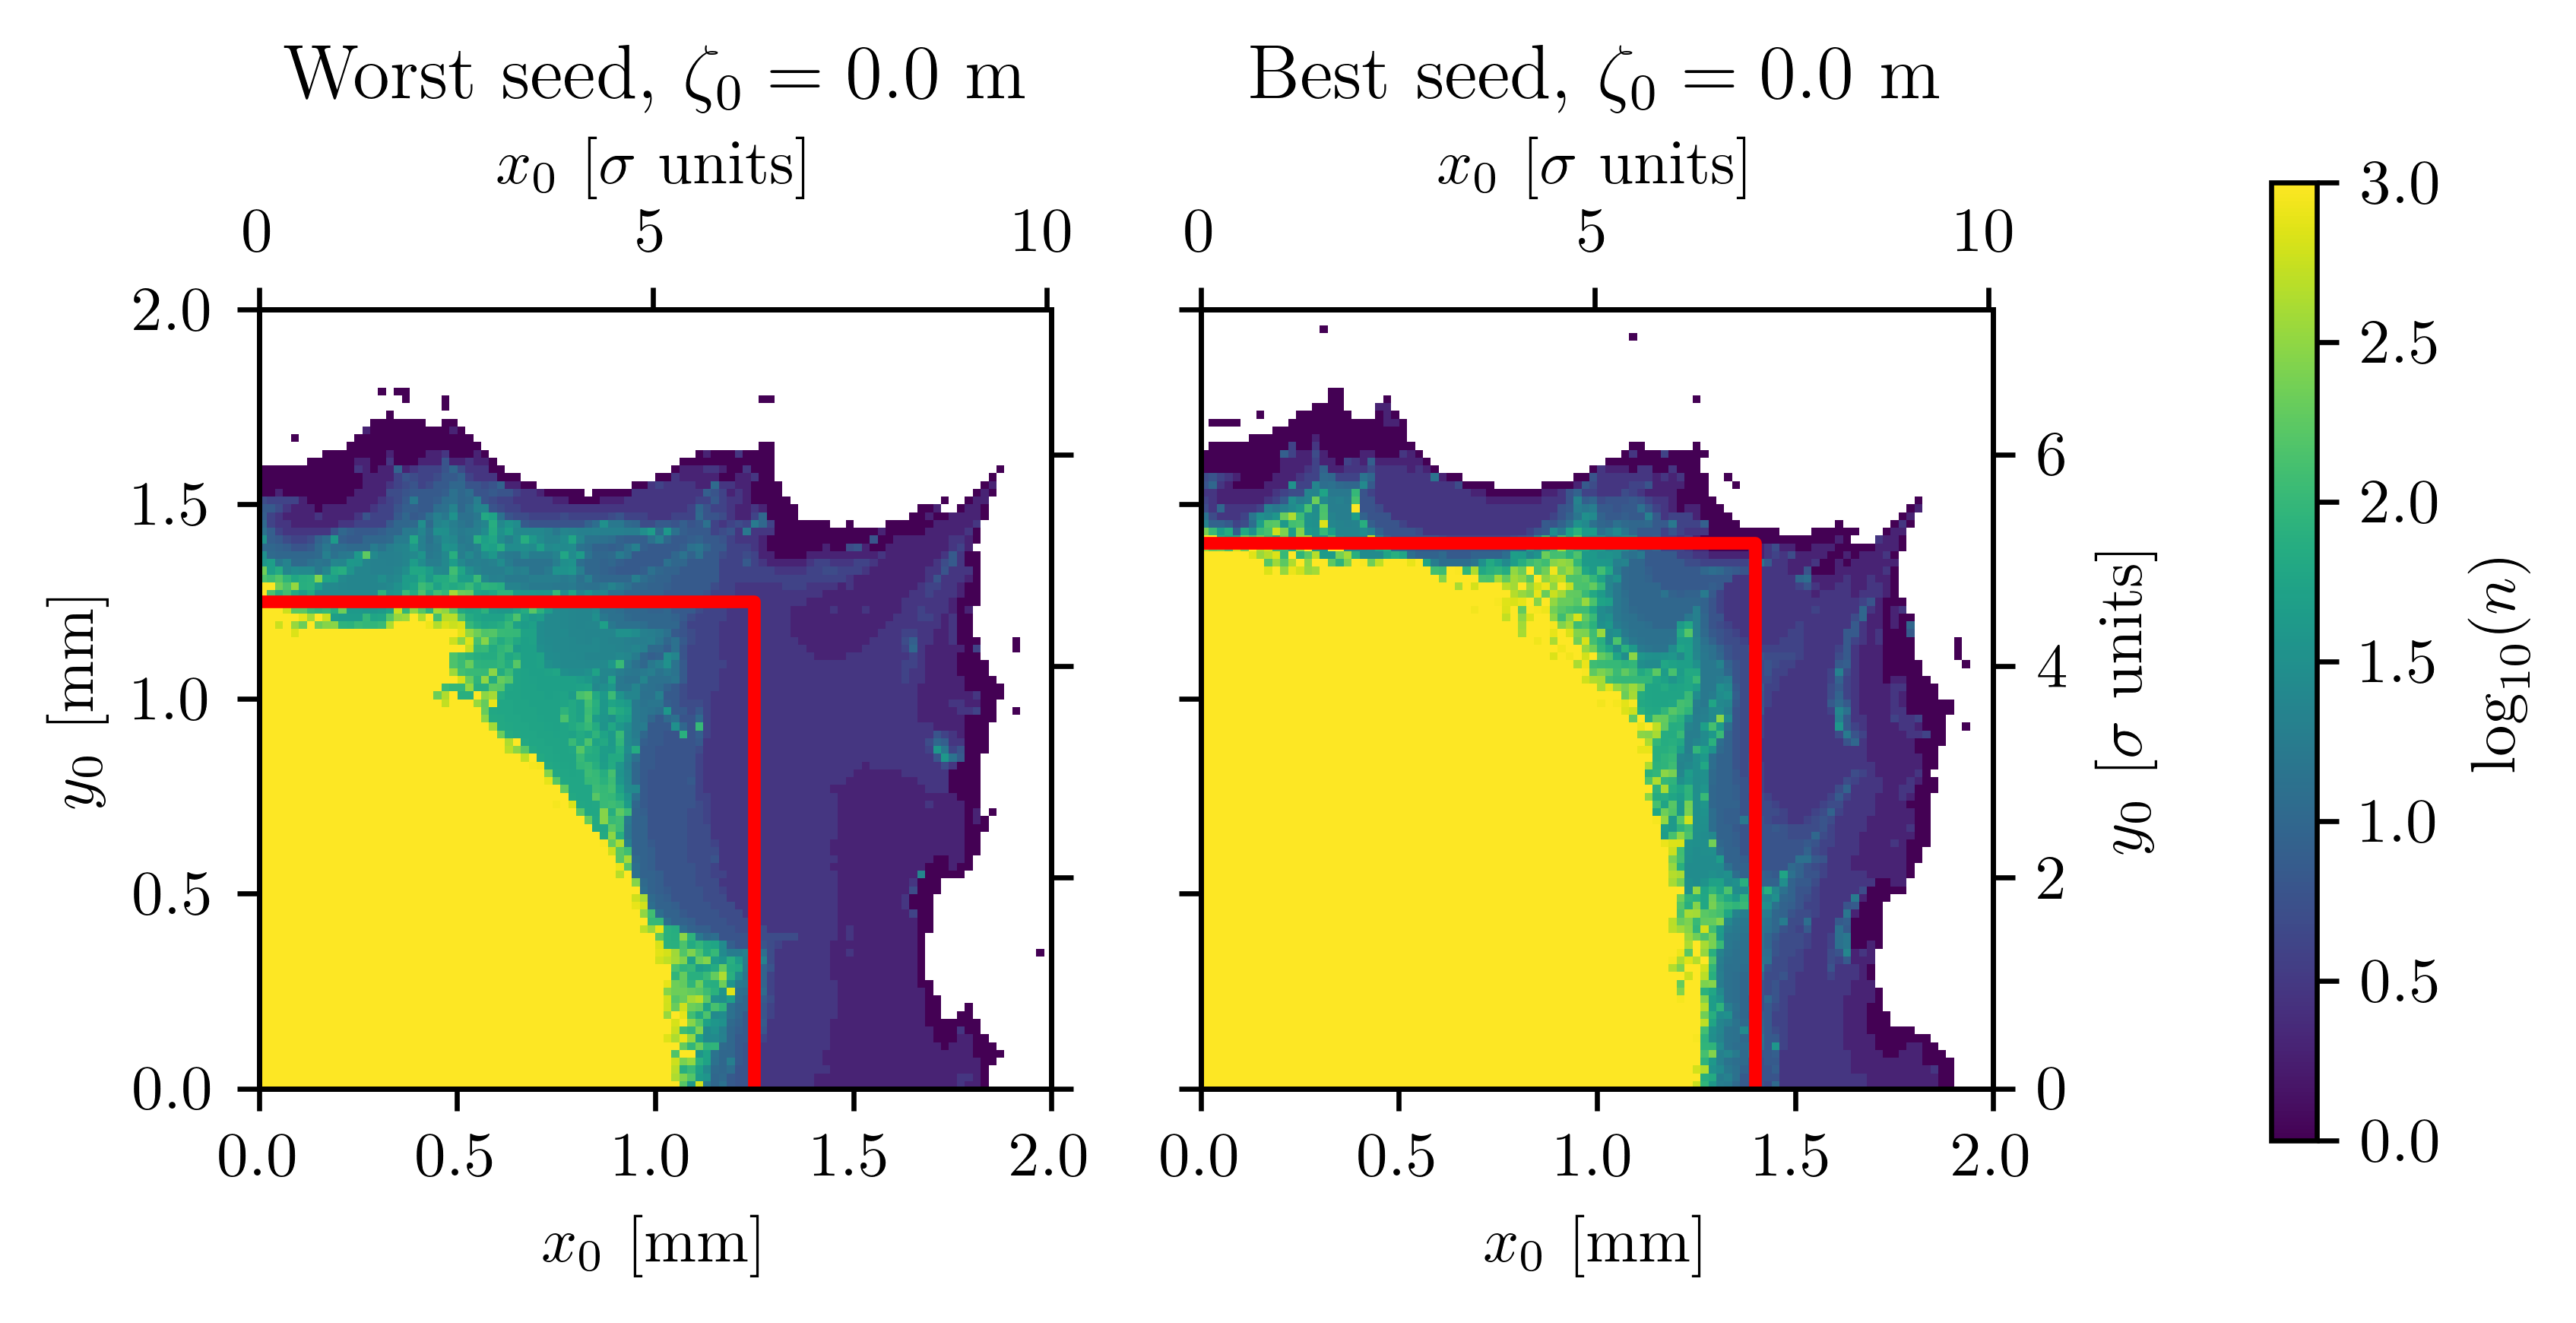
\includegraphics[width=\textwidth]{6_lhc_dynamic_indicators/figs/quick_scan.png}
    \caption{Survival plot up to $n=10^3$ turns of two different seeds of a realistic HL--LHC lattice of Beam 1, without beam-beam interaction, at \SI{7.0}{TeV}. The two seeds achieved, the worst and best dynamic aperture value out of the selection of 60 seeds available. The scan of initial conditions consists of $100\times100$ samples over a uniform Cartesian grid over the $x-y$ transversal plane. A region of interest (ROI) is highlighted in red on the two survival plots, and represents the choice of boundaries for the finer sampling we performed for our dynamic indicator analysis.}
    \label{fig:seed_presentation}
\end{figure}

To inspect the performance of the dynamic indicators, we sampled initial conditions on a uniform Cartesian grid of $300\times300$ particles in the $x-y$ transverse plane, with transverse moments $p_x$ and $p_y$ set to zero. The boundaries of the Cartesian grid were hand-picked based on the scan results presented in Fig.~\ref{fig:seed_presentation}, in order to have a square region of interest (ROI) focused on the dynamic aperture region highlighted at $n=10^3$. The ROI selected is highlighted in red.

The longitudinal variable $\zeta$ was set at three different values to inspect different levels of modulations, respectively, at \SI{0.0}{\meter}, at \SI{0.15}{\meter}, which is halfway close to the bunch separatrix, and at \SI{0.30}{\meter}, which is close to the bunch separatrix. See Fig.~\ref{fig:the_bunch} for an illustration of the $\zeta$ values chosen, which are based on the tracking results of multiple initial conditions with different initial $\zeta$ value and $x, p_x, y, p_y$ set to zero. This tracking yielded similar results for all seeds; therefore, this set of choices for $\zeta$ was identical for all selected lattices.

\begin{figure}
    \centering
    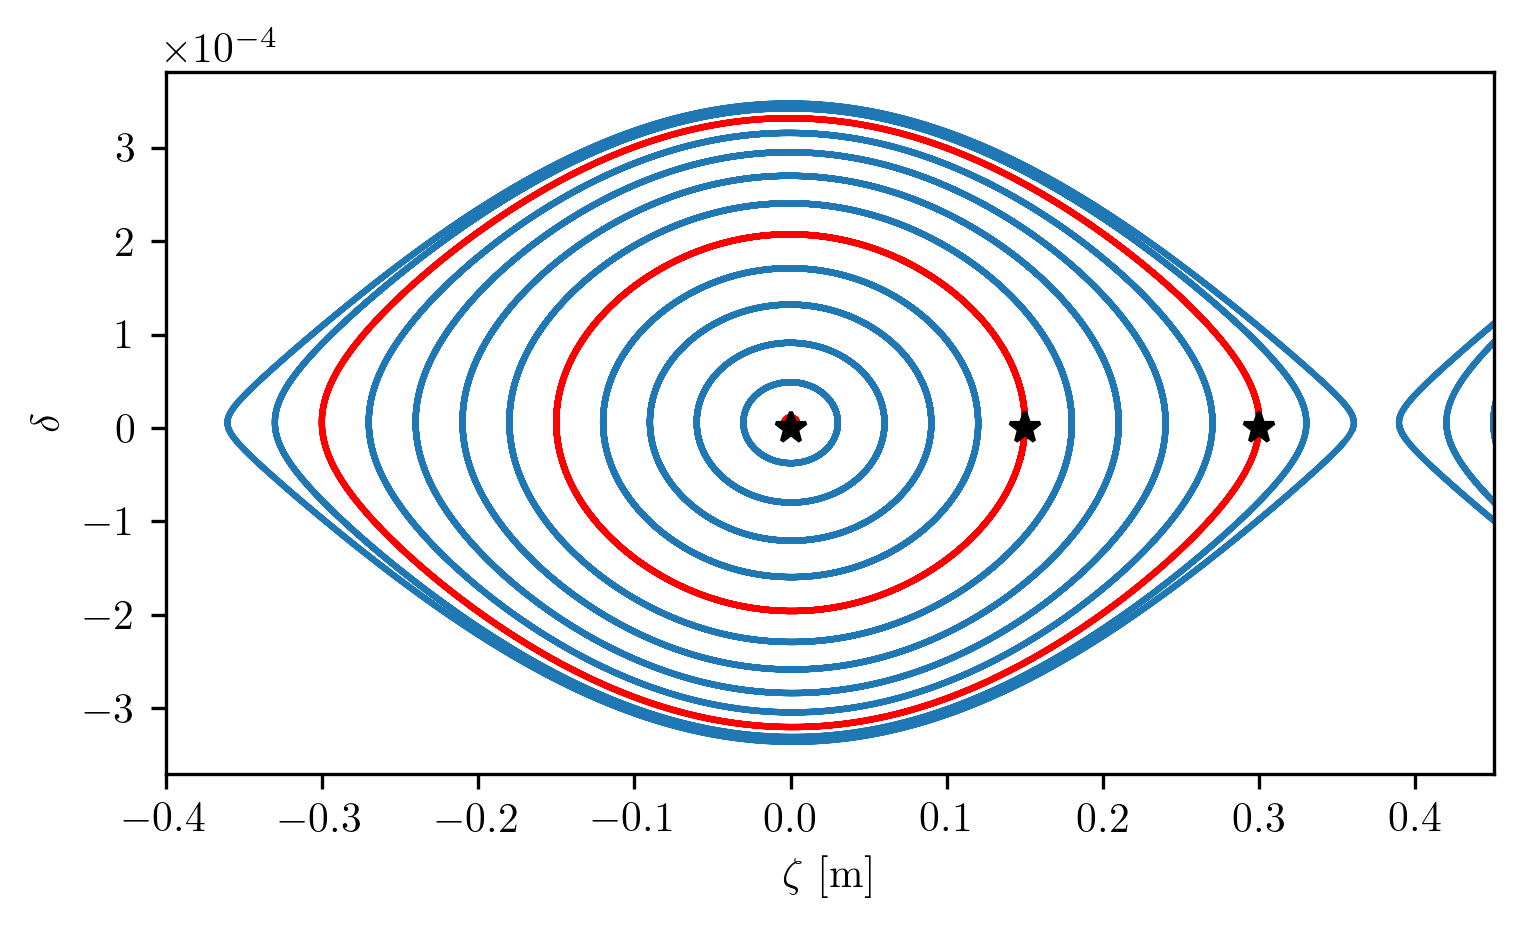
\includegraphics[width=0.65\textwidth]{6_lhc_dynamic_indicators/figs/longitudinal.png}
    \caption{Tracking of initial conditions with different $\zeta$ values up to $n=10^3$ on the HL-LHC lattice with median seed. The tracking highlights the classic bunch structure and shows that the separatrix is placed at $\zeta \gtrsim$ \SI{0.35}{\meter}. The three red crosses represents the three choices of $\zeta_0$ we decided to inspect in our dynamic indicator study.}
    \label{fig:the_bunch}
\end{figure}

\section{Results of numerical studies} \label{sec:results}

The dynamic indicators presented in the previous section, namely, $FLI/n$, $FLI^{WB}$, $GALI^{(k)}$, $REM$, and $FMA$, were evaluated on the HL-LHC lattices up to $n=10^5$ turns. The results of the evaluation of these indicators are presented in the following sections. Note how in general we will inspect the indicators at the median seed, as it is the seed that is most representative of the HL-LHC lattice features.

Note also how we present all the value distributions in logarithmic scale, as the indicators are expected to follow either a power law distribution or an exponential one, and the logarithmic scale allows us to better inspect the tails of the distribution and the general tendencies of these indicators to create bimodal distributions, with the sole exception of $FMA$, which, as we have seen from the results in the previous Chapter when considering a modulated Hénon map, tends to generate a tri-modal distribution.


\subsection{Overview of the chaotic regions of the HL-LHC lattice}

The inspected $300\times300$ Cartesian grid of initial conditions considered in the selected ROIs gives us an overview of the phase space ranging from zero amplitude to around 3.5 $\sigma$ units of amplitude.

An initial overview on how the phase space is structured can be seen in Fig.~\ref{fig:true_survivors}, where we report a survival plot for all six configurations of HL-LHC and $\zeta_0$ considered, tracked up to $n=10^5$ turns. As $n$ increases, a progressive erosion-like process of the region where particles are still not lost happens. This phenomenon is well known in literature, and it was studied for the development of dynamic aperture scale-laws, based on the Nekhoroshev theorem~\cite{}, which describe an exponentially slow decrease of dynamic aperture.

We can now inspect these same six HL-LHC configurations with dynamic indicators, and see what structures they highlight within the region where particles survive up to $n=10^5$ turns. In Fig.~\ref{fig:fli_all}, we report a colormap of the values of $\log_{10}(\mathrm{FLI}(\hat{x})/n)$ evaluated on the six configurations. We can see, as expected, how chaotic regions, corresponding to the higher values of the indicator, occur at the borders of the stable region, showing for the case of certain configurations isolated structures that resemble islands of stability, with regular initial conditions within, these structures can be related to nonlinear resonance effects~\cite{}. Conversely, the internal core region is fully constituted by initial conditions with regular behaviour.

\begin{figure}
    \centering
    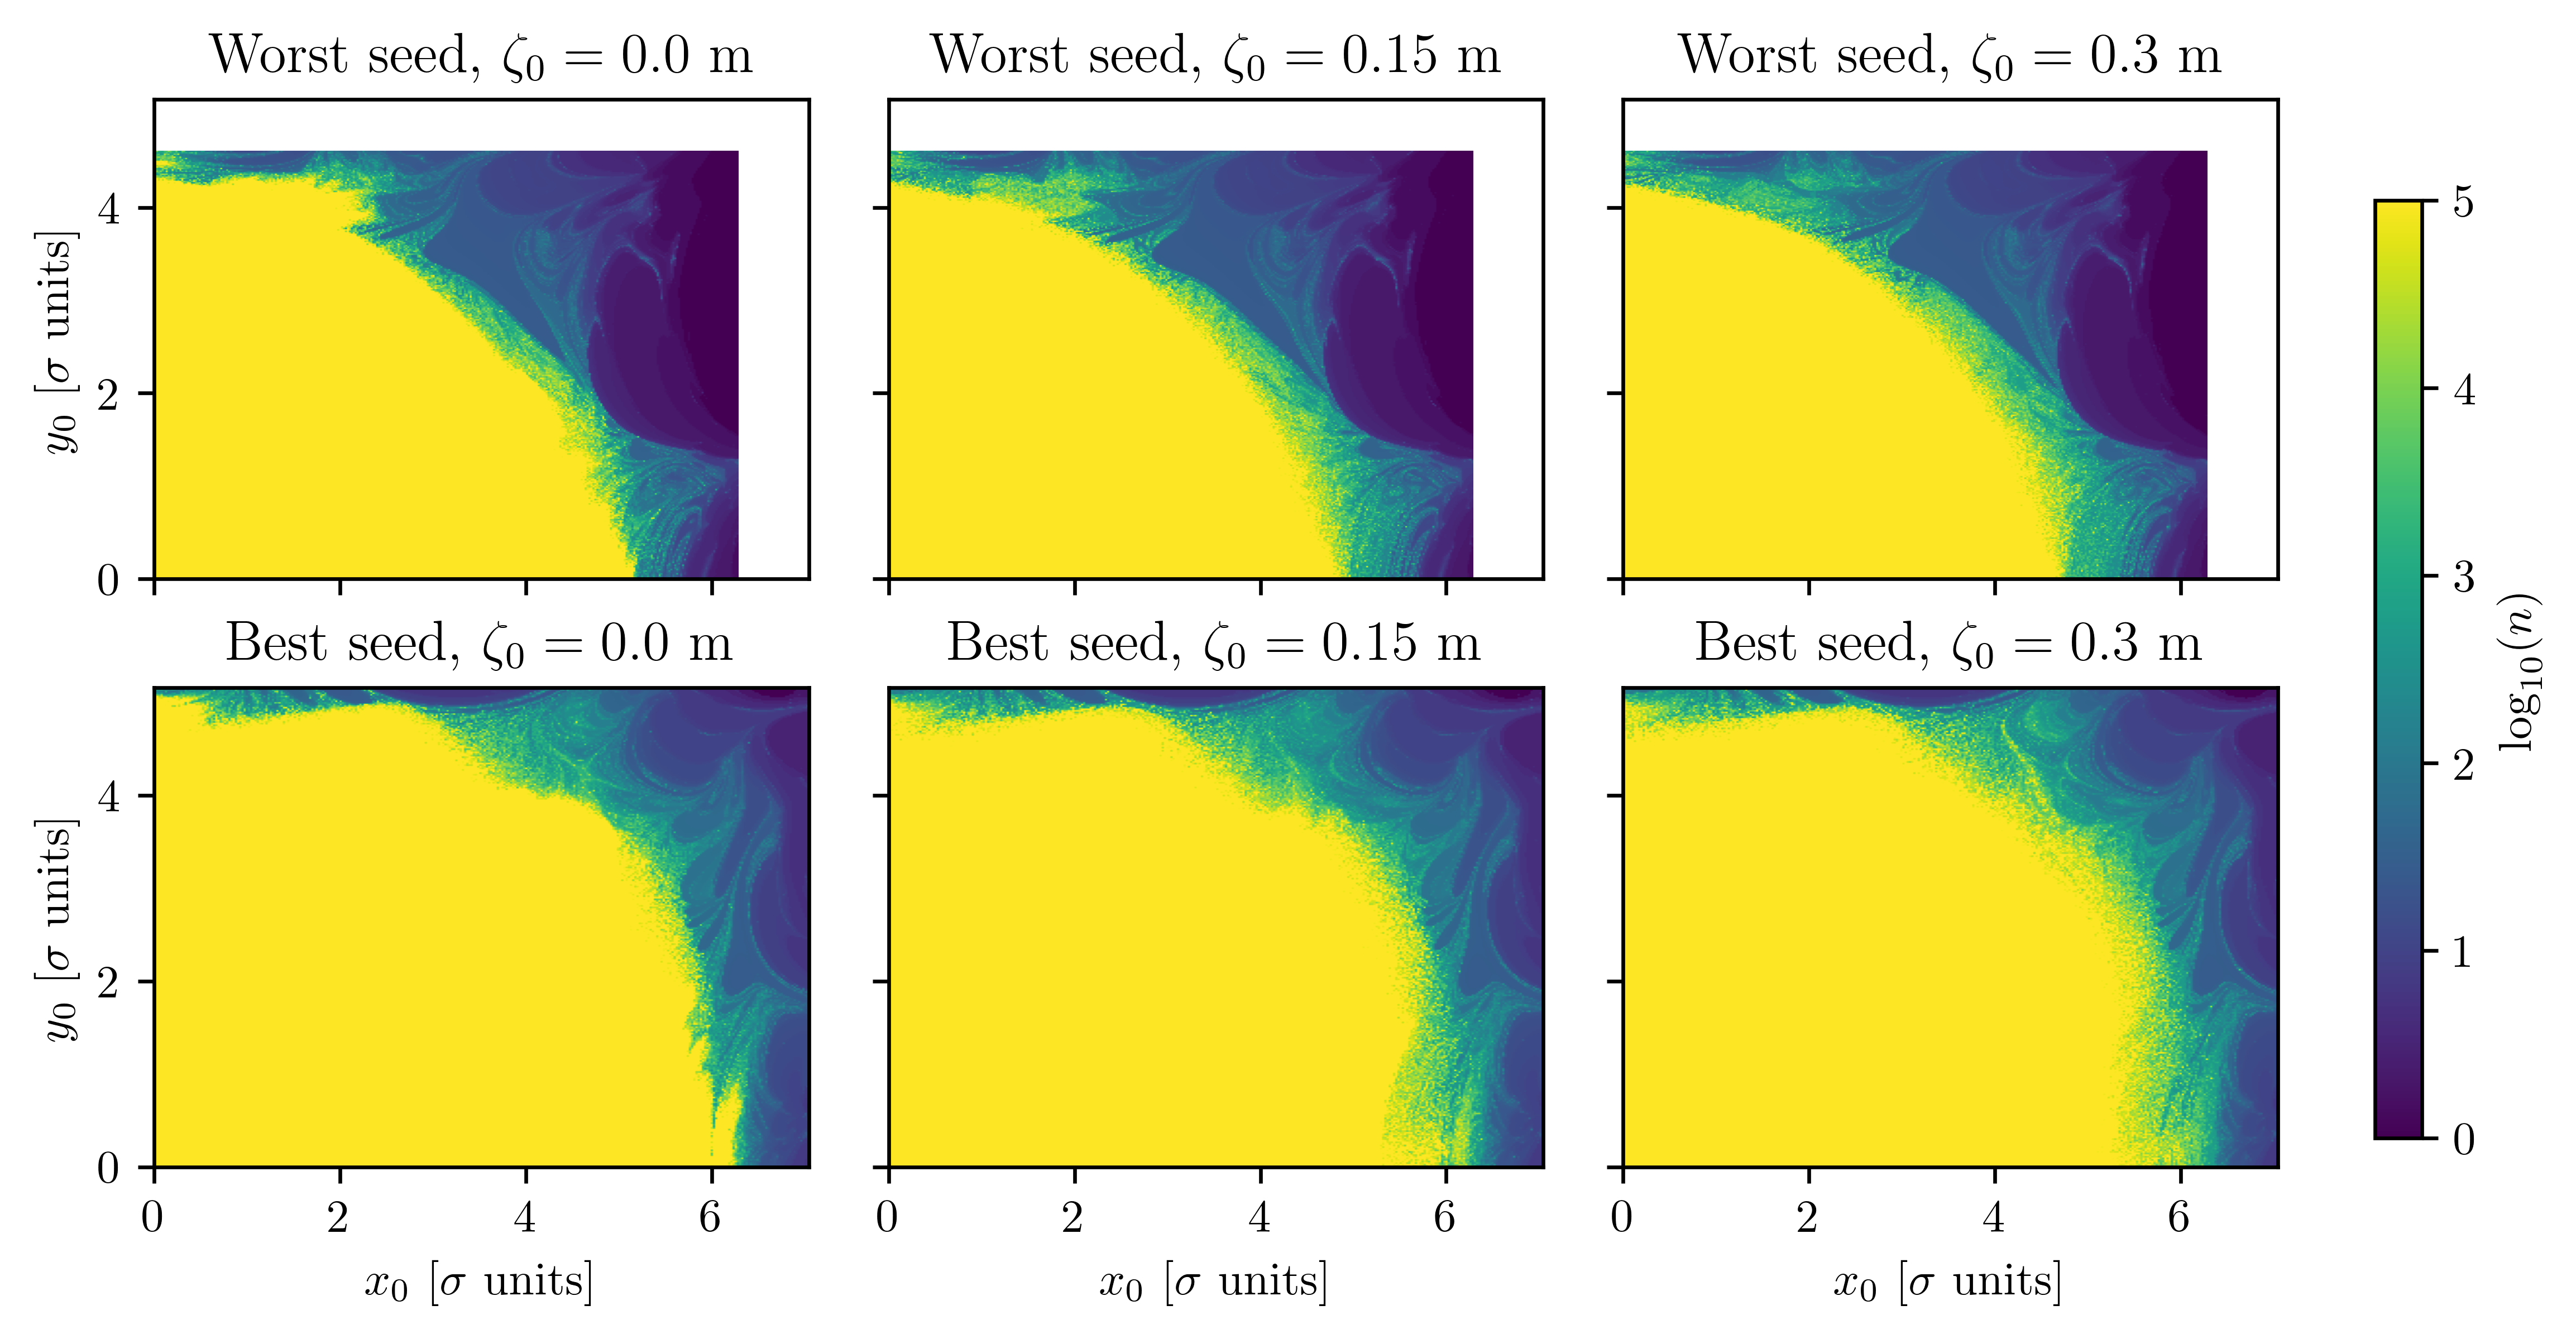
\includegraphics[width=1.0\textwidth]{6_lhc_dynamic_indicators/figs/stability.png}
    \caption{Survival plot up to $n=10^5$ turns for all nine configuration of the realistic HL-LHC lattice model considered.}
    \label{fig:true_survivors}
\end{figure}

\begin{figure}
    \centering
    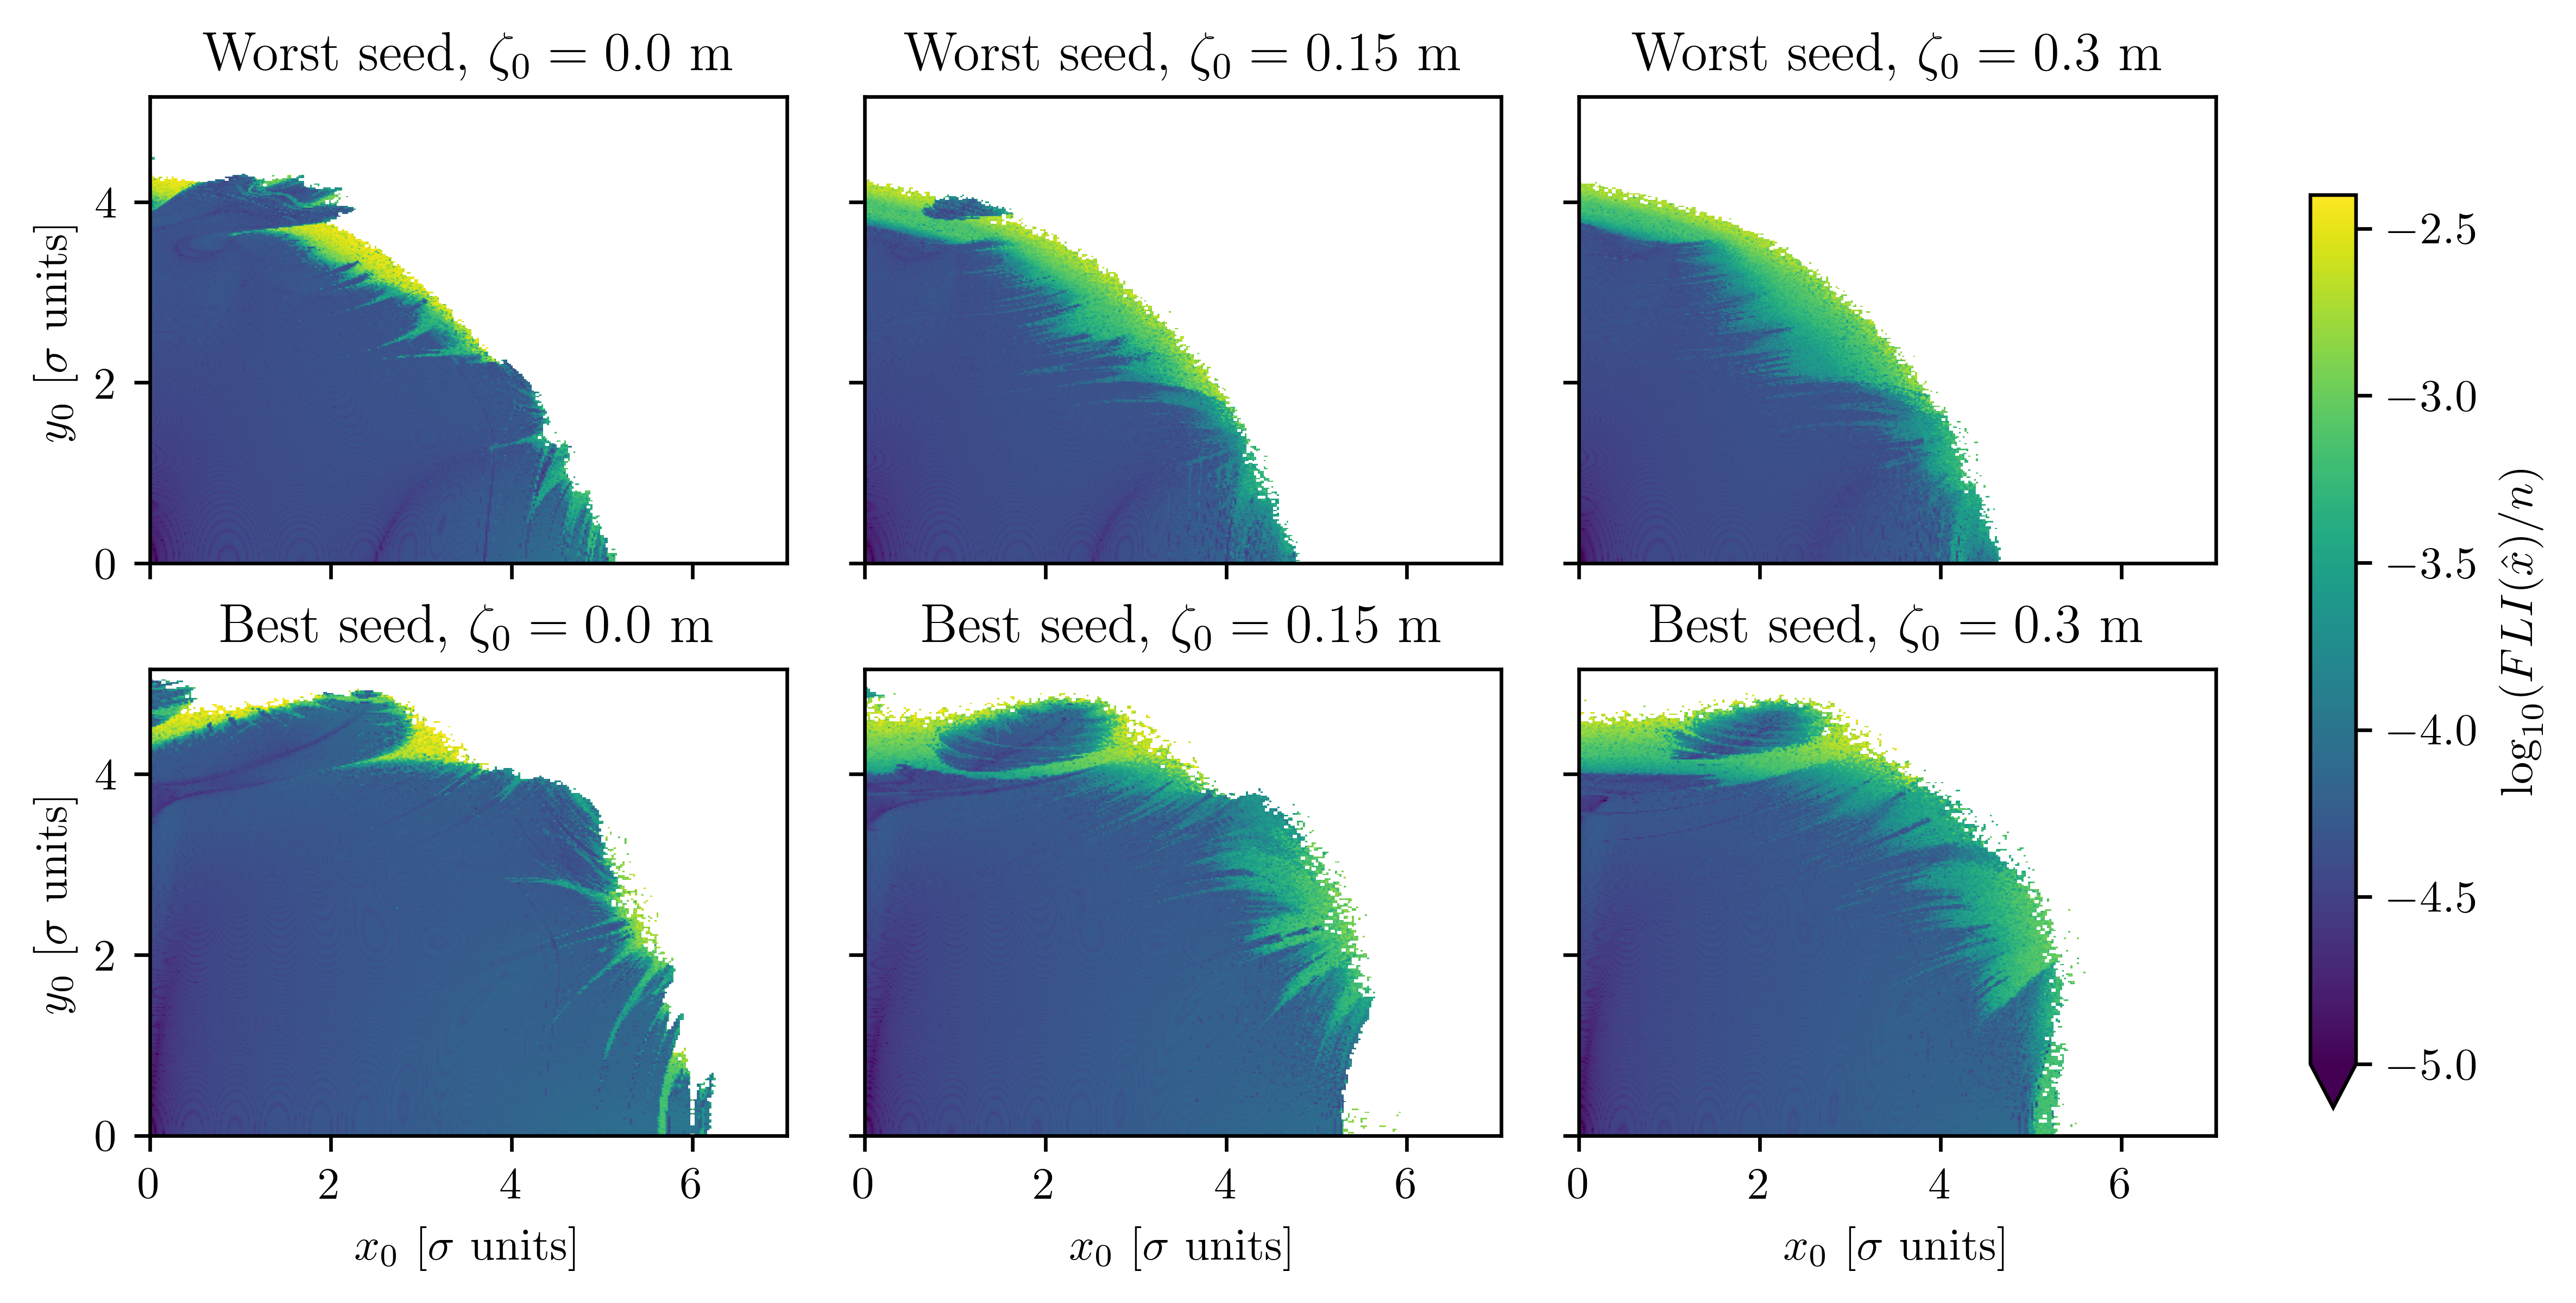
\includegraphics[width=1.0\textwidth]{6_lhc_dynamic_indicators/figs/fli_all.png}
    \caption{$\log_{10}(\mathrm{FLI}(\hat{x})/n)$ evaluated at $n=10^5$ for all nine configuration of the realistic HL-LHC lattice model considered.}
    \label{fig:fli_all}
\end{figure}

The size and shape of the chaotic regions appears to be dependent both from the noise seed and the initial value of $\zeta_0$. The worst performant seed also features larger regions of chaos in the phase space, while the best performant has the smallest one among the three inspected. We can see also how the increase of $\zeta_0$ contributes to slightly enlarge the size of chaotic regions, as the introduction of stronger longitudinal dynamics causes more modulation effects in the transverse plane, leading to more chaotic initial conditions. 

While it is expected to see in the various lattices a correlation between the presence of large chaotic regions and a faster dynamic aperture decrease over time, we must stress out that it is not an always correct approach, nor the target of this paper, to seek out a direct connection between the Lyapunov exponent of an initial condition and its stability time, as it is well known that exceptions to such connections, such as stable chaotic initial conditions, or regular unstable initial conditions, do exist~\cite{}.

However, it is of interest to inspect the average value of the Lyapunov time (that is, the inverse of the maximum Lyapunov exponent~\cite{}) at different amplitudes. In Fig.~\ref{fig:evo_fli_nek}, we plot the inverse value of FLI$/n$, evaluated at $n=10^5$, over increasing amplitude. We can see how the values follow an exponential-like scale law. This functional shape resembles a Nekhoroshev-like scale law~\cite{}, which found multiple applications in the definition of dynamic aperture scale laws.

In Fig.~\ref{fig:overview}, we present an overview of the various dynamic indicators in analysis evaluated for one of the HL-LHC lattices, in the form of colormaps evaluated at $n=10^5$. We can see how the various dynamic indicators, with the exception of $FMA$, tend to highlight the same regions of chaos, giving overall a coherent evaluation of the phase space. The exception given by $FMA$ will be commented in a later Subsection. 

In Fig.~\ref{fig:overview2}, instead, we present an overview of the evolution of the value distribution of the various dynamic indicators for different $n$ values. We can see how, in general, the dynamic indicators tend to converge into a bimodal distribution, with the sole exception of $FMA$, which instead converges into a tri-modal distribution. This tendency has been documented for Lyapunov exponent distributions in~\cite{}, and it has been used in~\cite{} as the main feature for benchmarking the classification performance of dynamic indicators.

\begin{figure}
    \centering
    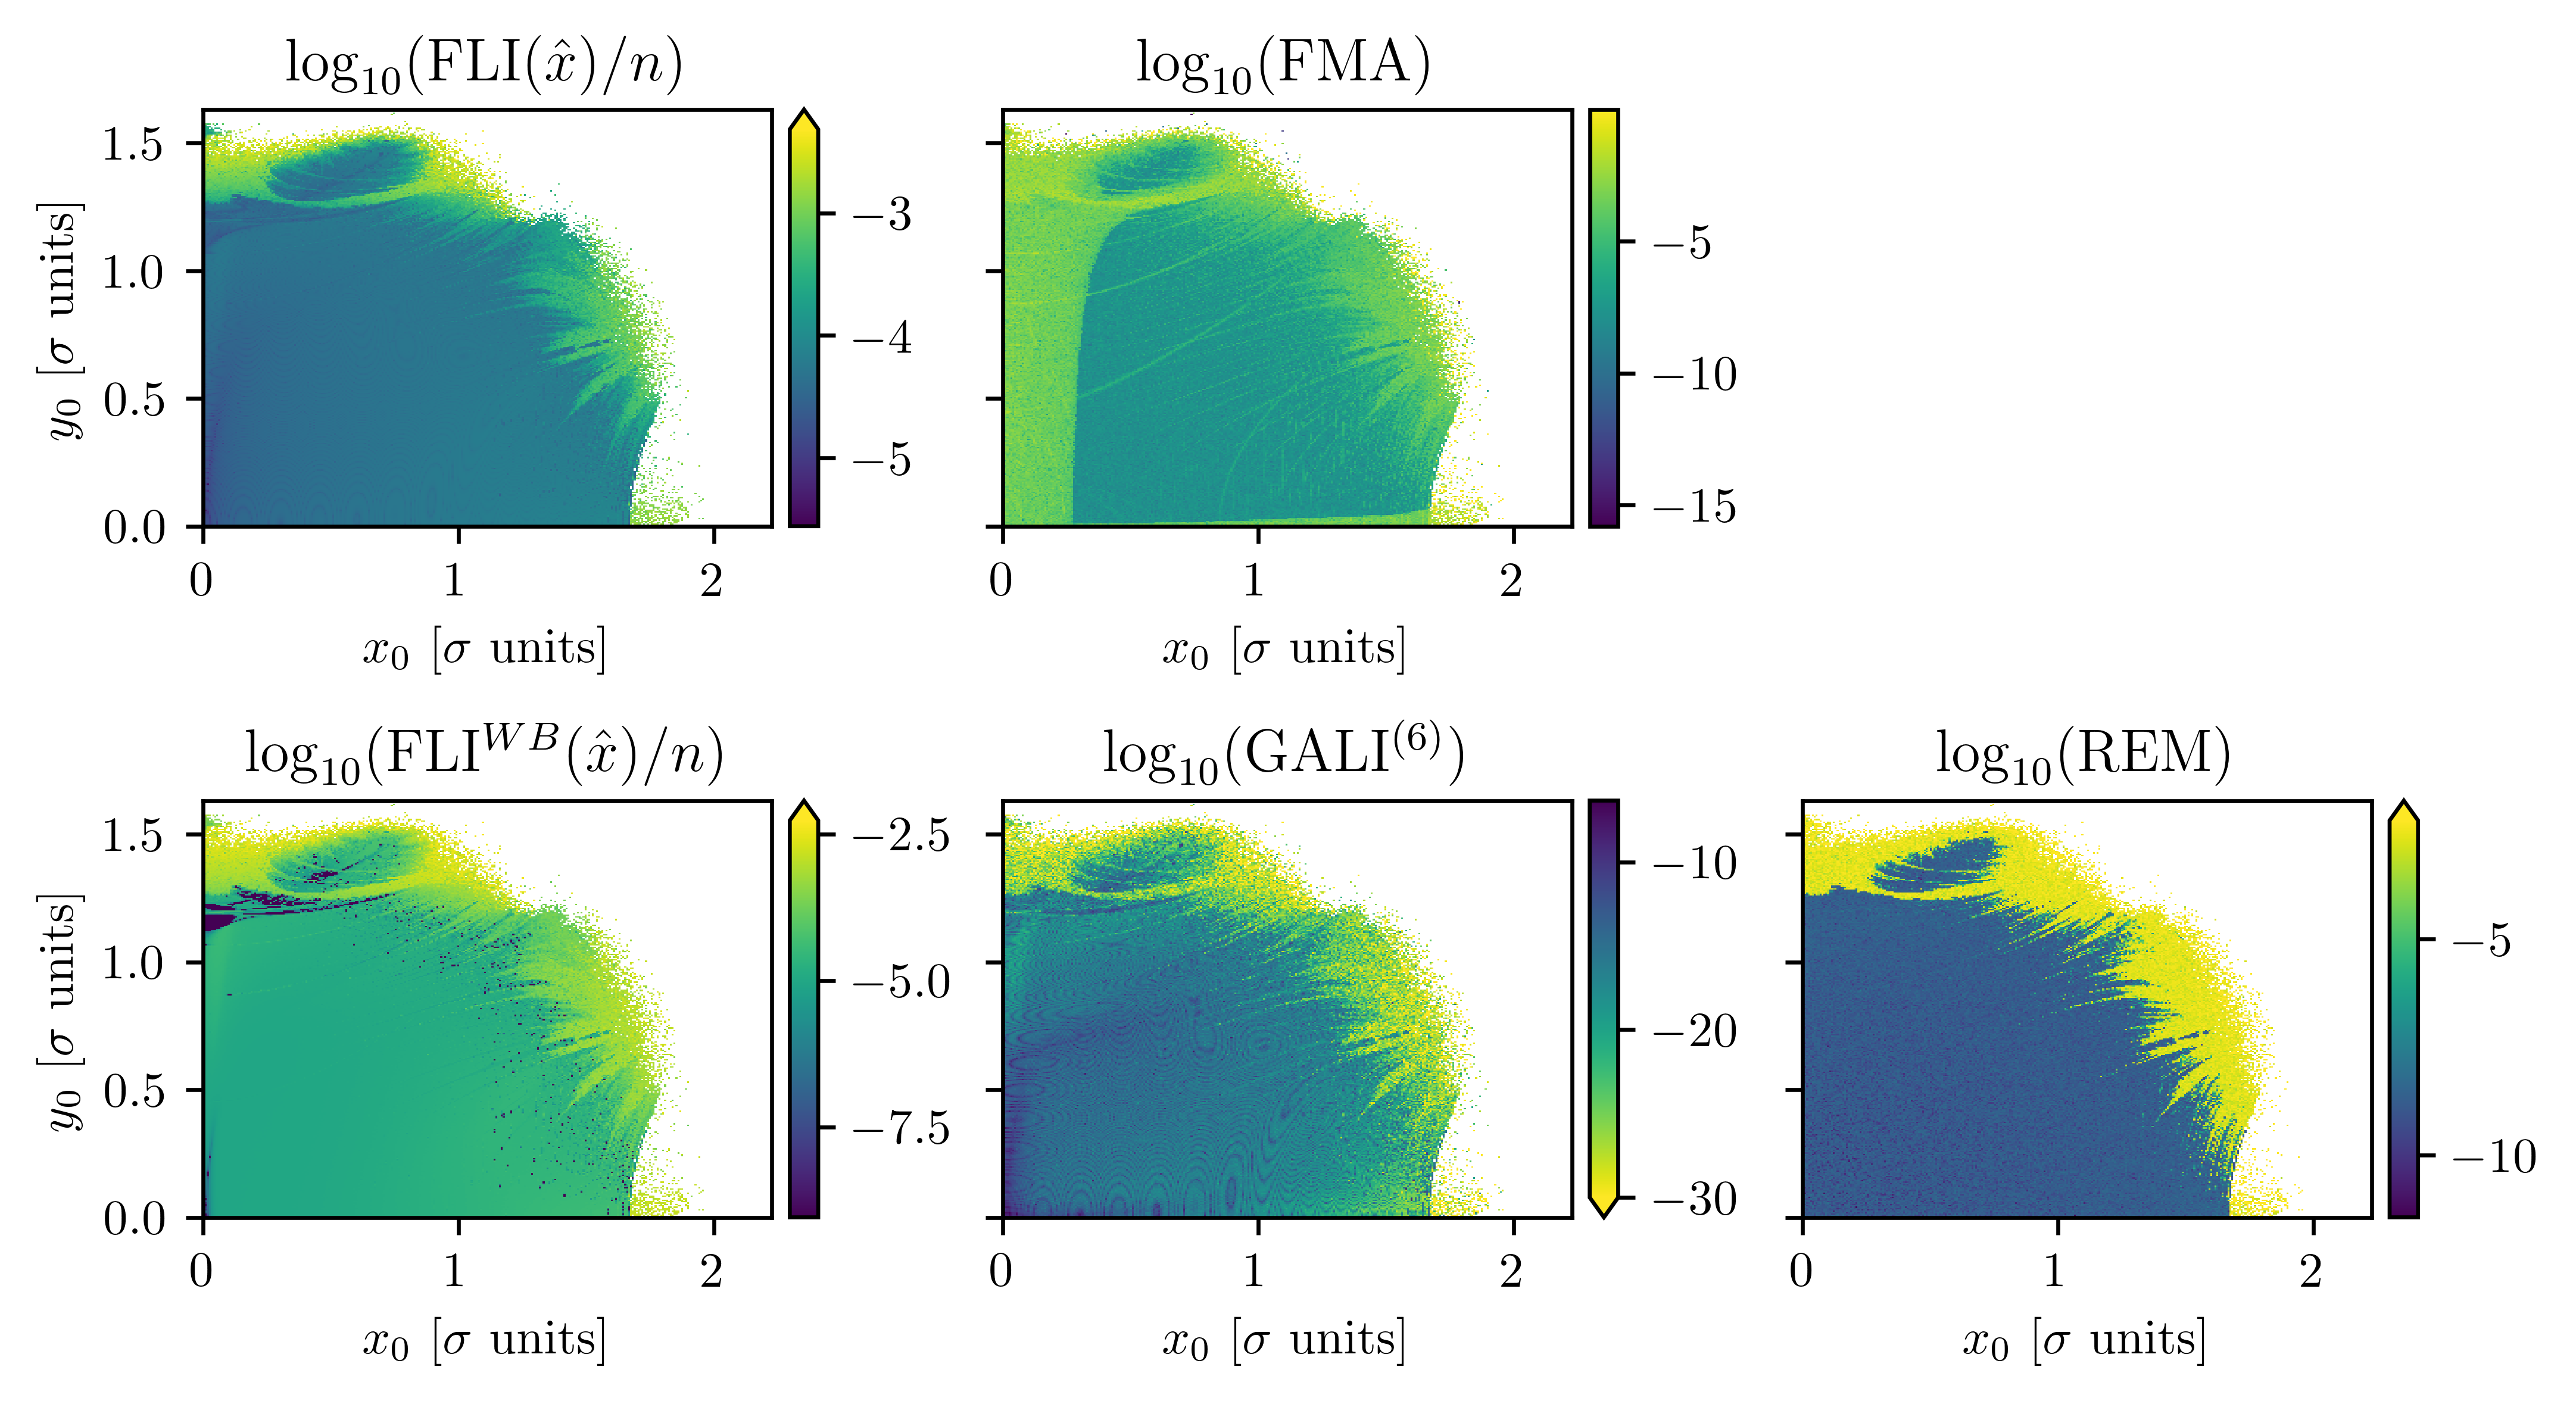
\includegraphics[width=1.0\textwidth]{6_lhc_dynamic_indicators/figs/overview.png}
    \caption{Color maps of the various dynamic indicators for a realistic HL-LHC lattice, evaluated at $n=10^5$. It can be seen how the indicators globally highlight the same structures in phase space, with the exception of $FMA$, which also shows additional structures. (HL-LHC lattice used: median seed, $\zeta_0=$\SI{0.15}{\meter}.)}
    \label{fig:overview}
\end{figure}

\begin{figure}
    \centering
    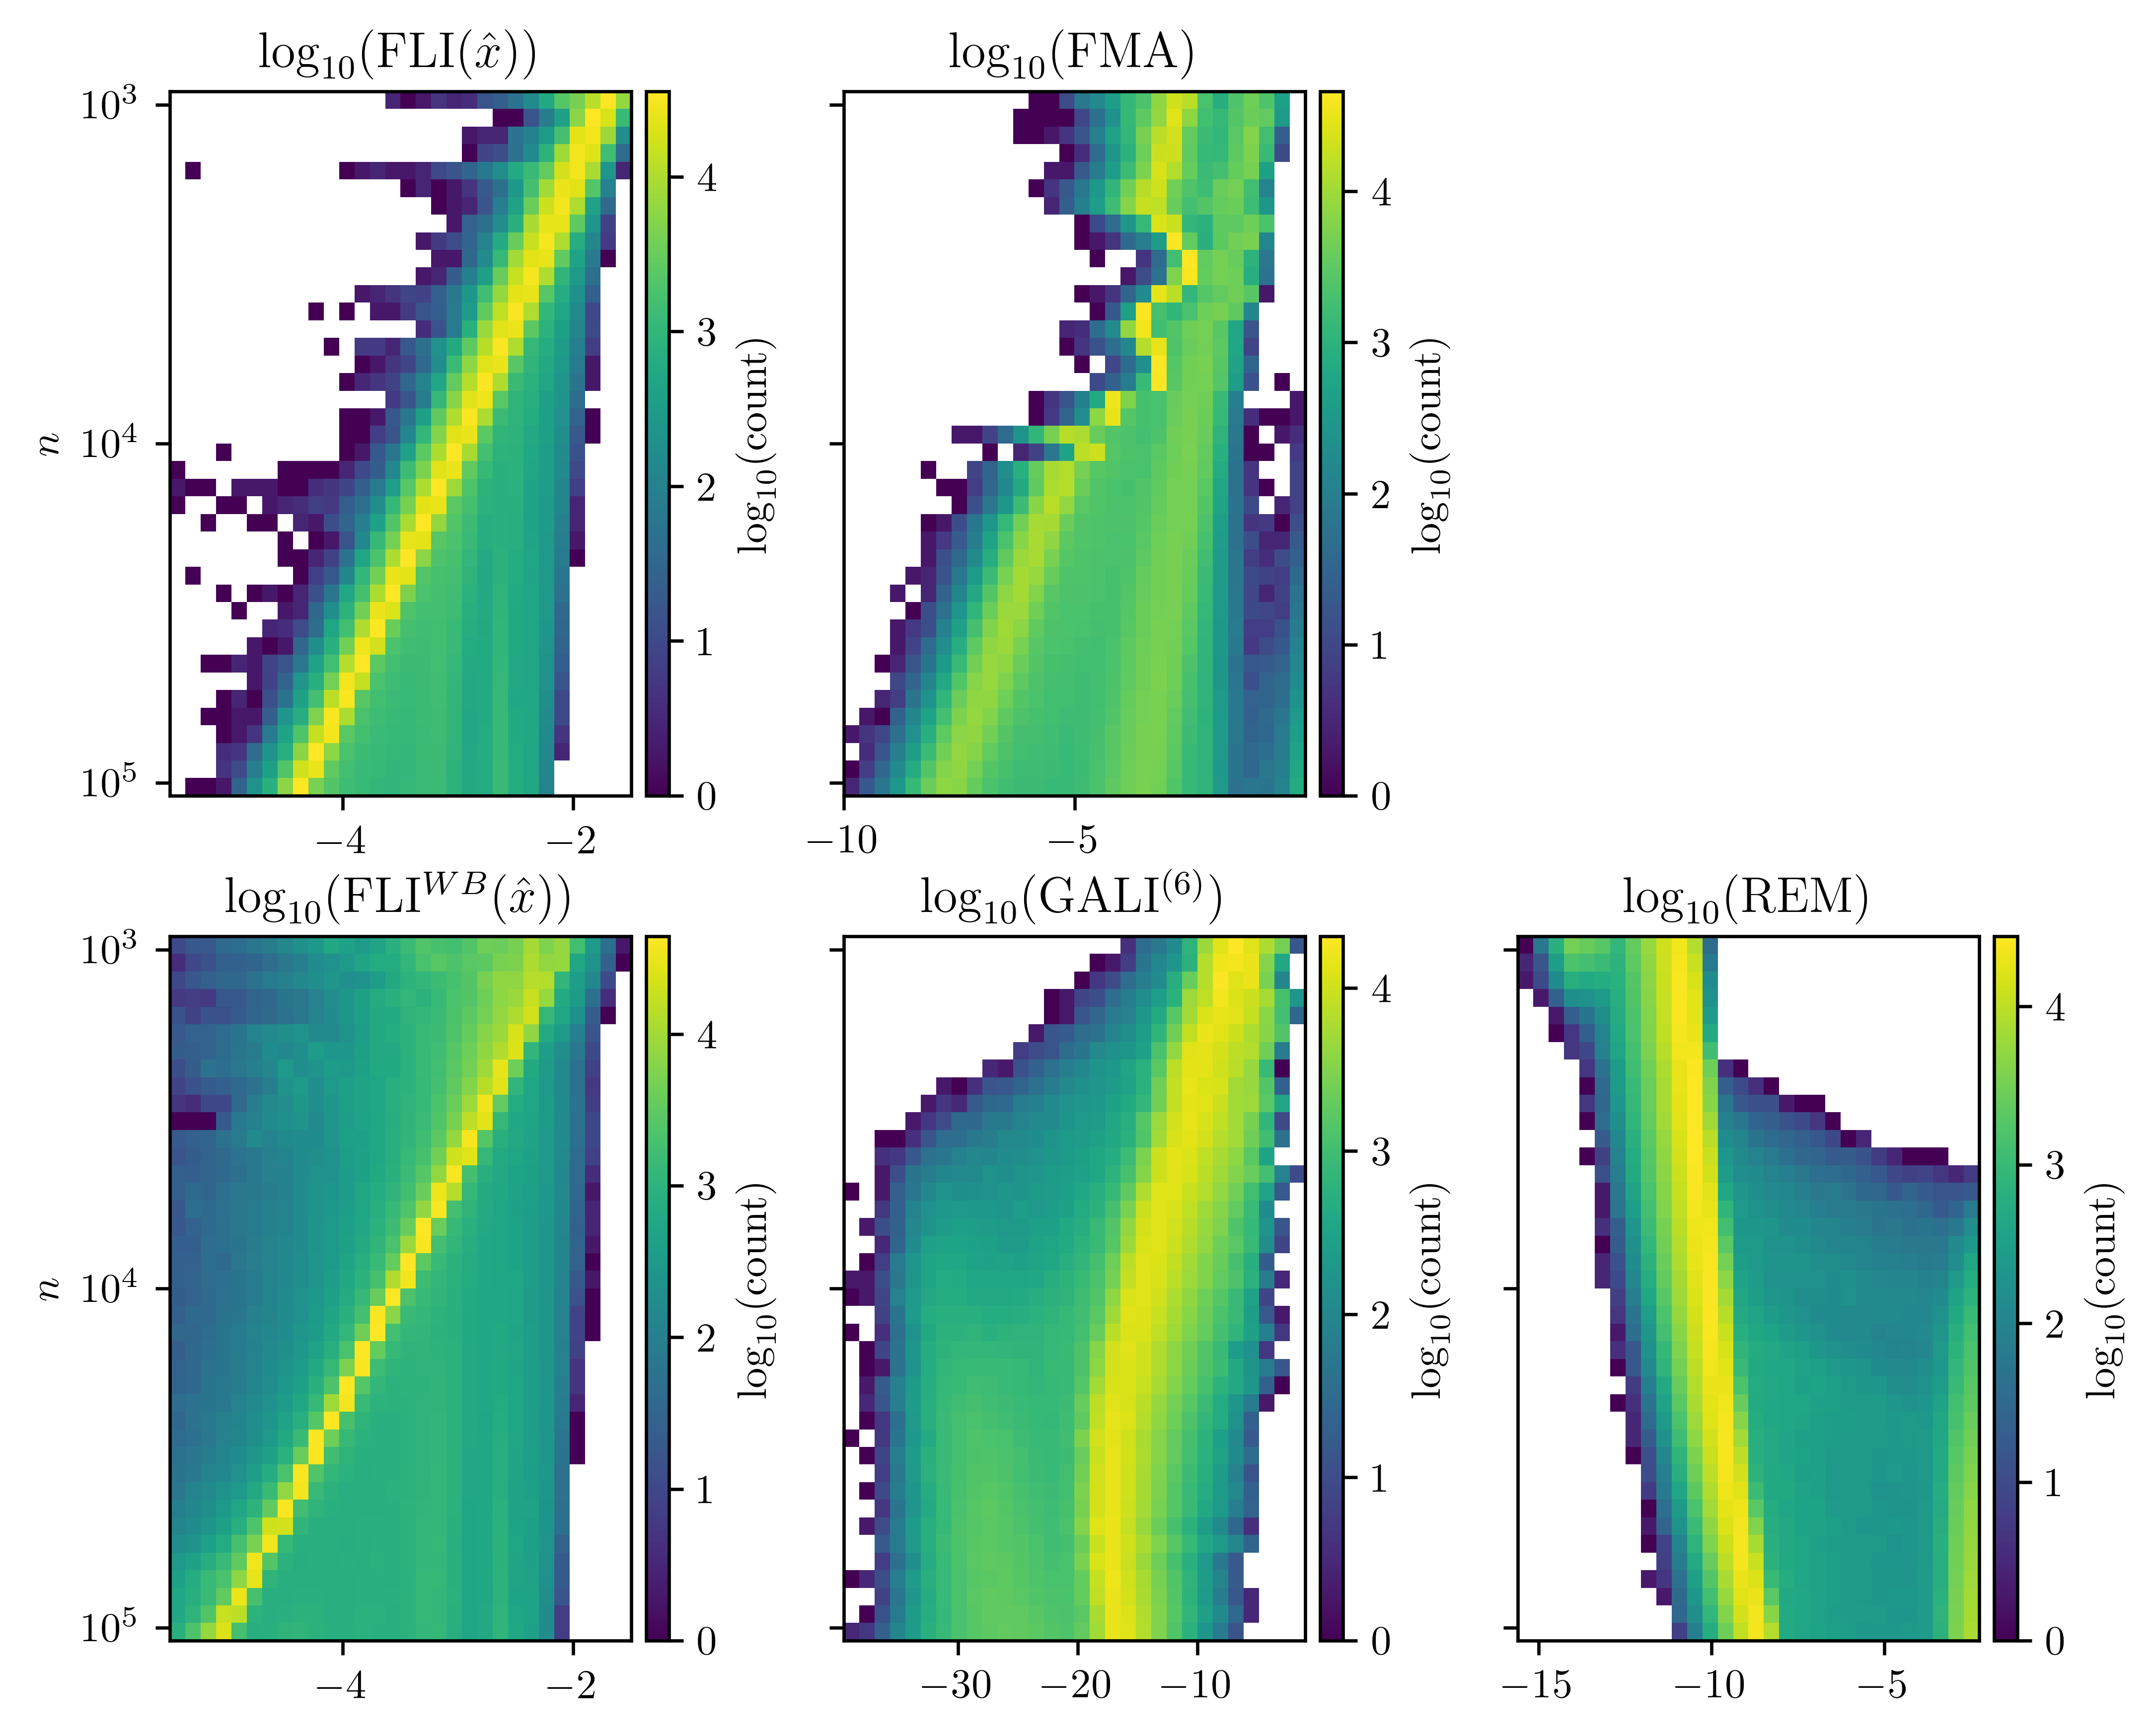
\includegraphics[width=1.0\textwidth]{6_lhc_dynamic_indicators/figs/evolution.png}
    \caption{Distribution of values of the various dynamic indicators as a function of time for a realistic HL-LHC. For low values of the number of turns $n$, the distribution is in general represented by a uni-modal function. For higher values of $n$, we can see the formation of either two separate clusters, making the distribution bi-modal, or an individual cluster with a significant tail. $\log_{10}(FMA)$ constitutes an exception, as it evolves forming a tri-modal distribution. (HL-LHC lattice used: median seed, $\zeta_0=$\SI{0.15}{\meter}.)}
    \label{fig:overview2}
\end{figure}

\subsection{$FLI$ dependence from the initial displacement}

$FLI$, by definition, is dependent from the initial choice of direction of the unitary displacement vector $\vb{\xi}$. This implies that initial choices of direction of the displacement vector can lead to the highlight of different structures in the phase-space.

To assess the magnitude of such differences, in Fig.~\ref{fig:fli_compare}, we compare the calculated values of $\log_{10}({FLI})$, calculated at $n=10^5$ with an initial displacement along one of the six orthonormal vectors, namely $\hat{x},\,\hat{p}_x,\,\hat{y},\,\hat{p}_y,\,\hat{\zeta},\,\text{and }\hat{\delta}$. The comparison is done against the mean value computed on the six possible initial displacement. The standard deviation is also presented.

It is possible to see how the different choice of initial displacement highlights different structures in the regular region, while chaotic regions tend to assume the same final value. This difference is highlighted also by the standard deviation evaluation, as the chaotic regions at the border show in general a low standard deviation, while the stable regions at lower amplitude have higher values.

This result is to be expected, as chaotic initial conditions are characterised by a strong maximal Lyapunov exponent, which leads different initial displacements to eventually align along it after a high enough number of turns. While, conversely, regular initial conditions might do not exhibit this preferential direction and lead to higher differences in $FLI$ values for different initial conditions. It's important to highlight, however, the fact that the general character of the dynamic indicator stays consistent along the various directions, and at most causes slight evaluation differences for the initial conditions close to the border between a regular and a chaotic region in the phase space.

\begin{figure*}[htp]
    \centering
    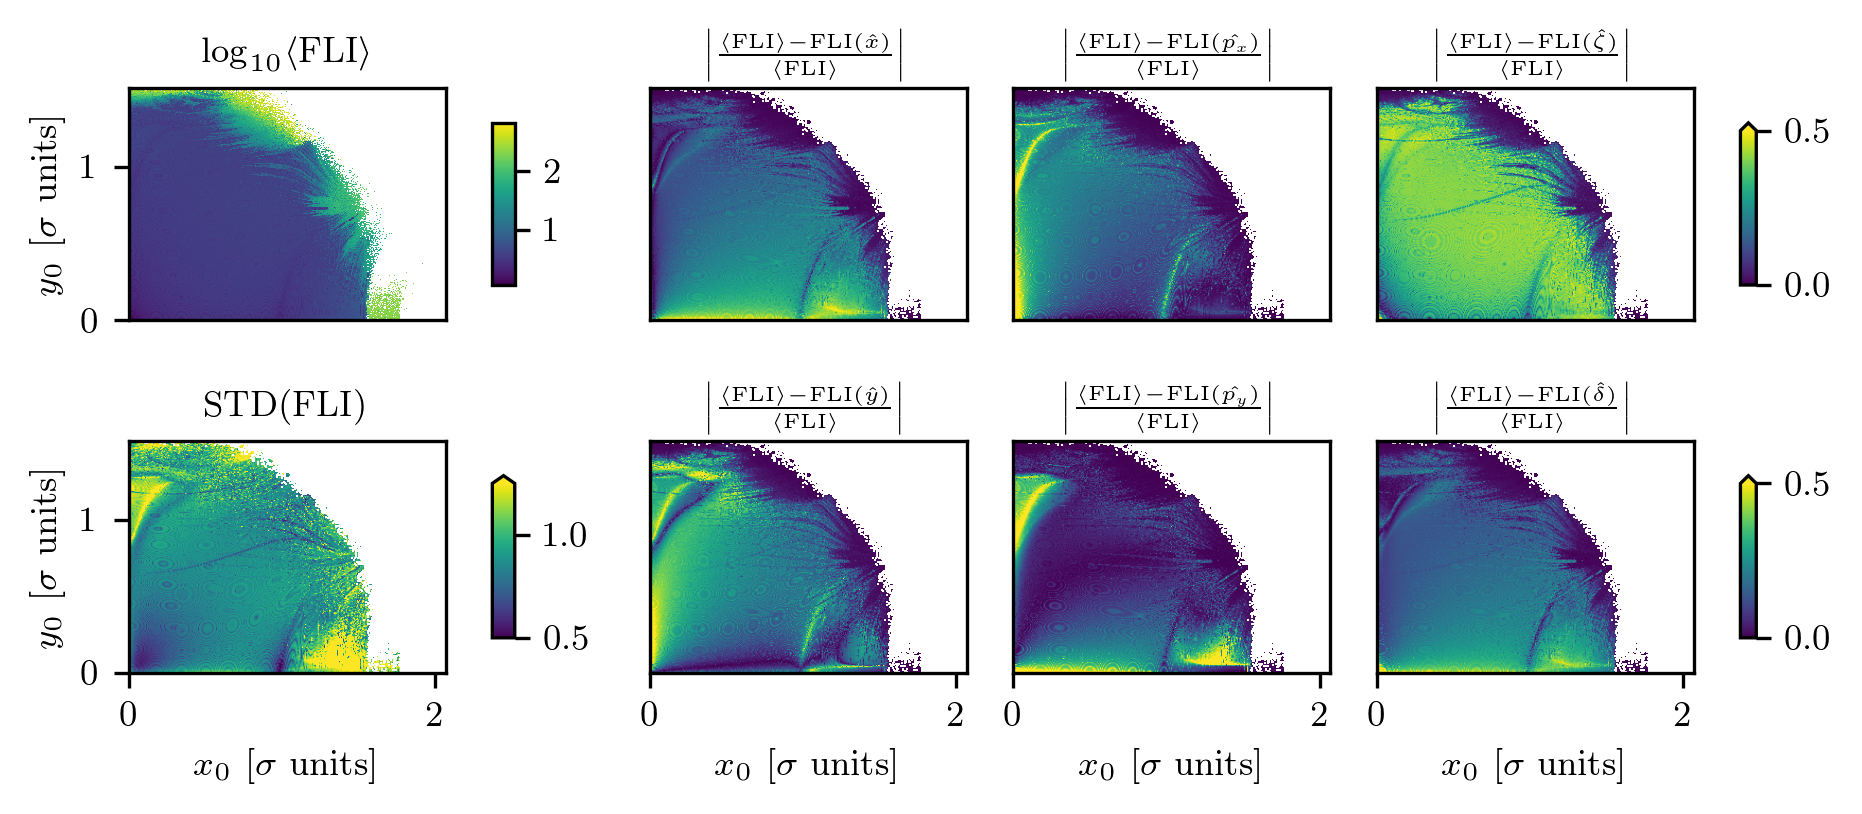
\includegraphics[width=1.0\textwidth]{6_lhc_dynamic_indicators/figs/fli_mean_std.png}
    \caption{}
    \label{fig:fli_compare}
\end{figure*}

\subsection{Application of Birkhoff weights to $FLI$}

To quantify the convergence improvements given by the Birkhoff weights, we compare the values obtained for $FLI$ at different times for one of the HL-LHC lattices, using either the standard approach that considers the mean in Eq.~\eqref{eq:fli_mean}, that is, $FLI/n$, or the weighted mean based on the use of Birkhoff weights as in Eq.~\eqref{eq:fli_birkhoff}, that is, $FLI^{WB}$.

In this analysis, we consider two ensembles of regular and chaotic particles, that have been classified by means of the value of the $FLI$ indicator computed for $n=10^5$ turns. In this context, we consider as regular particles the ones that have archived a final value of $\log_{10}(\mathrm{FLI}/n) < -4.5$, and as chaotic particles we consider the ones that have archived a final value of $\log_{10}(\mathrm{FLI}/n) > -2.5$. This arbitrary thresholding is based on the expected properties of the dynamic indicator $FLI$, and considers a subset of initial conditions that have manifested either clear regular or chaotic behaviour already at $10^5$ turns, while excluding the ones that still do not have a clear classification.

The sets are then used to calculate the time evolution of both $FLI/n$ and $FLI^{WB}$, in order to evaluate possible classification improvements in the latter compared to the first. These improvements can be for example an increase convergence rate in values or an increased spread between the values of regular initial conditions and chaotic initial conditions.

In Fig.~\ref{fig:fli_compare_mean_birk} (left), the comparison between the two indicators is made for a subset of the set of regular initial conditions, whereas on the right we show the comparison for the subset of chaotic ones. It is possible to observe how, for regular initial conditions, Birkhoff averaging does not seem to significantly improve the convergence rates of the dynamic indicator, but it does introduce a gap that slightly improves the gap between regular and chaotic initial conditions, once the chaotic initial conditions reach saturation.

\begin{figure}[htp]
    \centering
    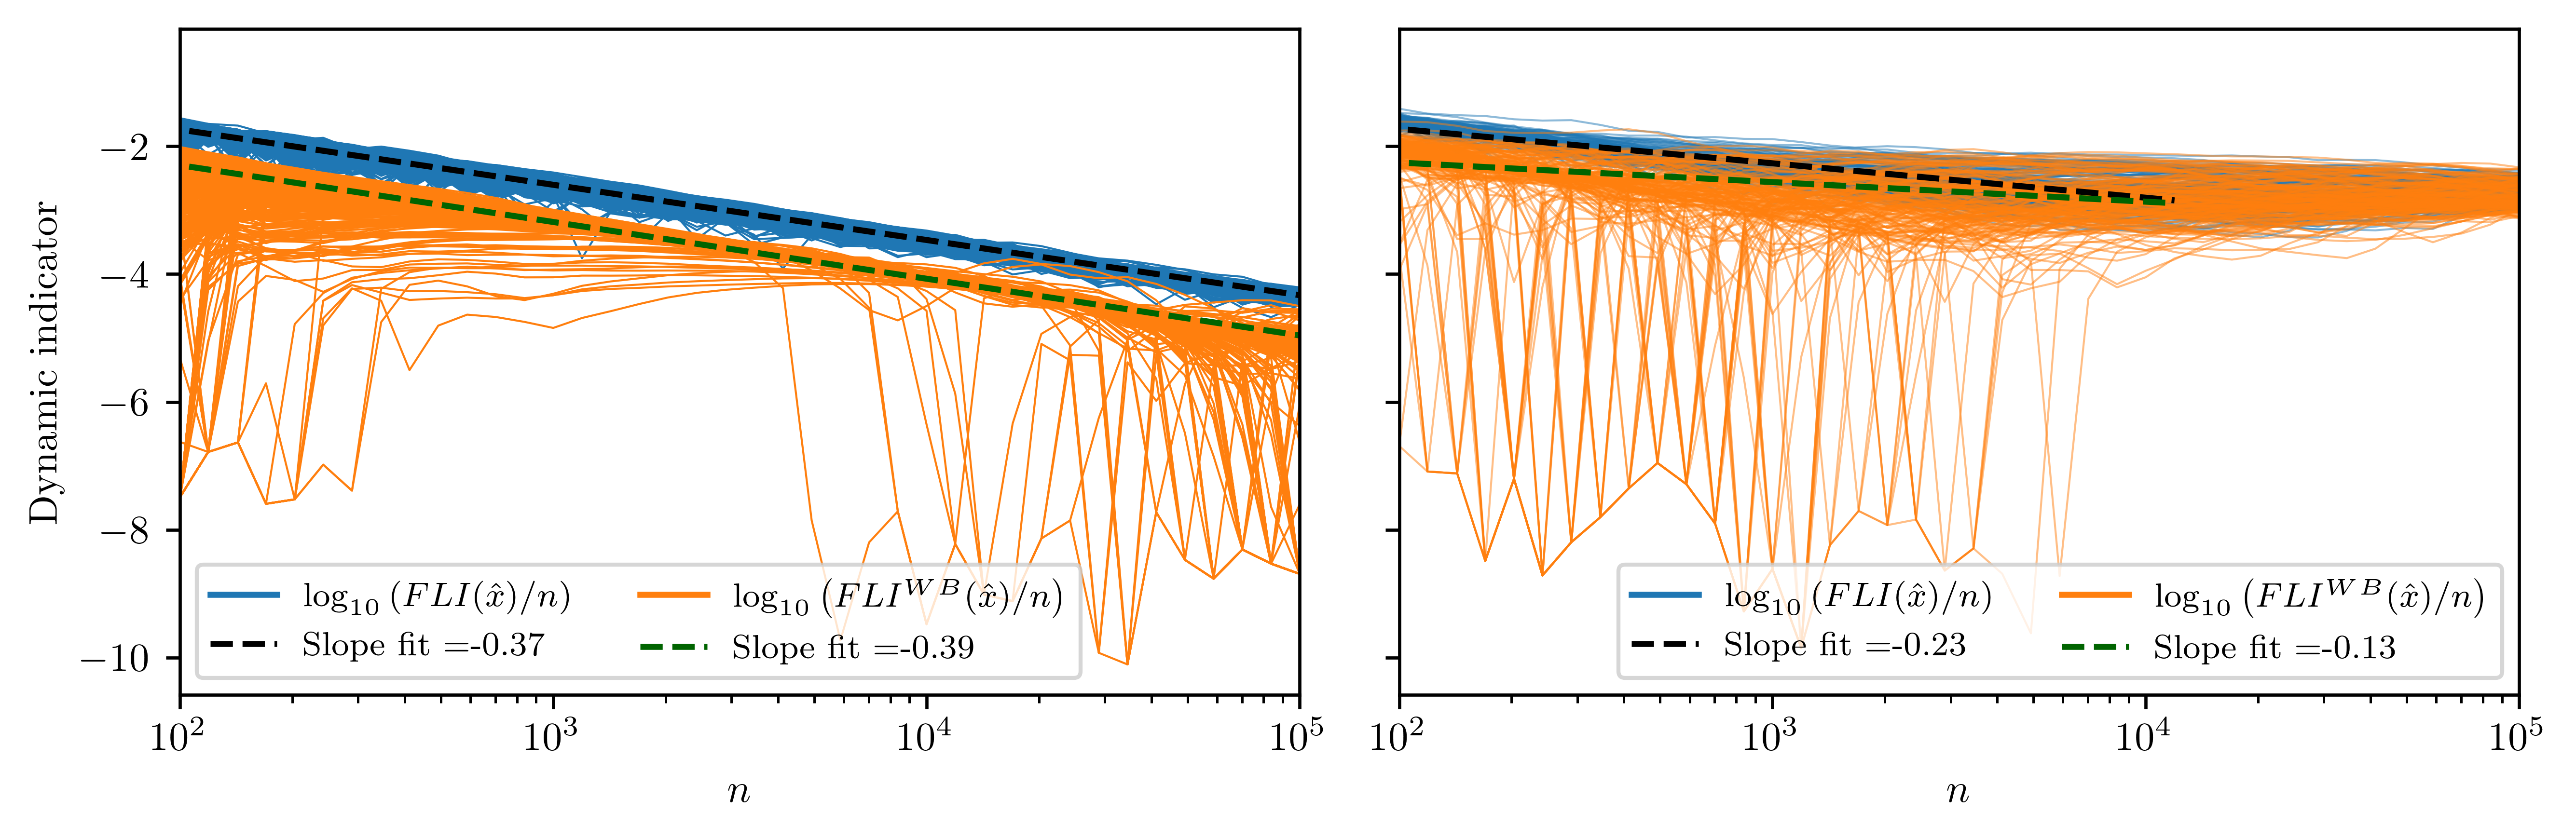
\includegraphics[width=1.0\textwidth]{6_lhc_dynamic_indicators/figs/fli_vs_flibk_idx_4.png}
    \caption{Time evolution of $FLI$ computed using either a standard mean ($FLI/n$) or the Birkhoff averaging ($FLI^{WB}$). Left plot: indicators computed for a set of 100 regular initial conditions, the fit highlights an almost identical convergence rate for the two averaging methods, although a gap between the evaluations is present. Right plot: indicators computed for a set of 100 chaotic initial conditions. A slight difference in convergence rate is observed for low $n$ values, before reaching a saturation value of the indicator of the order of $10^{-4}$. (HL-LHC lattice used: median seed, $\zeta_0=$\SI{0.15}{\meter}.)}
    \label{fig:fli_compare_mean_birk}
\end{figure}

For chaotic initial conditions, a saturation region is observed for the indicator value of the order of $10^{-4}$ for both indicators. When this value is reached, both indicators oscillate around it. However, the slope with which this non-zero value is reached is different for the two indicators and is higher in absolute value for $FLI^{WB}$ than for $FLI/n$. We must also point out how some chaotic initial conditions exhibited strong value fluctuations in $FLI^{WB}$ before the saturation point, reaching values comparable to the regular initial conditions. These isolated cases might be artefacts caused by the Birkhoff weights which amplify certain modes in the time series when the chaotic behaviour still has not fully manifested.

Despite these isolated oscillations in value, the improvement brought about by the Birkhoff averages can be appreciated in Fig.~\ref{fig:fli_colormap_mean_birk}, where the time evolution of the distribution of the values of $FLI/n$ (left) and $FLI^{WB}$ (right) is shown for the entirety of initial conditions evaluated for Fig.~\ref{}. The part of the distribution corresponding to the regular initial conditions reaches its peak (yellow band) and moves toward zero with increasing $n$. However, the displacement toward zero is sharper for $FLI^{WB}$, enabling better classification. In both graphs, a faint trace of a peak is visible corresponding to the indicator value of about $10^{-4}$. This feature is remarkably similar for the two indicators, as already seen in Fig.~\ref{fig:fli_colormap_mean_birk}.

When applied to a modulated Hénon map, as seen in Subsection~\ref{}, the Birkhoff weights applied to $FLI$ provided a slight improvement in the convergence of regular initial conditions to zero, as well as an overall benefit in highlighting the two separate clusters of initial conditions. In this context, such difference in convergence was not appreciated to a comparable extent, however, a slight improvement in cluster sharpness and separation was noted, suggesting that Birkhoff weights do still offer a slight improvement to $FLI$ classification. This can be appreciated by comparing the value distribution evolution of $\log_{10}(FLI/n)$ and $\log_{10}(FLI^{WB})$ reported in Fig.~\ref{}. There is also a possibility that an improvement in convergence can be observed only at higher values of $n$.

\subsection{Lyapunov time and stability time}

The Lyapunov time is the characteristic timescale on which an initial condition shifts to regular dynamics to chaotic dynamics. It is defined as the inverse of the system's maximal Lyapunov exponent, which is directly estimated by the dynamic indicators $FLI/n$ and $FLI^{{WB}}$.

We are interested in assessing whether this estimate of the maximal Lyapunov exponent can be used to assess the presence of a Nekhoroshev-like evolution in the system. In other words, we want to inspect if the estimated Lyapunov time follows a Nekhoroshev-like scale-law with the initial amplitude $I_0$ of an initial condition, such as the one in Eq.~\eqref{}.

This analysis is motivated by the well-known fact that dynamic aperture follows a Nekhoroshev-like evolution~\cite{}. The details of this functional relation have been presented in Subsection~\ref{}. As the Nekhoroshev scale-law describes an exponential decay of the estimate stability time of initial conditions as their initial amplitude $I_0$ grows, we expect to observe a similar behaviour for the Lyapunov time, and therefore to be able to use the Lyapunov time as an additional tool for assessing the presence of a Nekhoroshev-like evolution in the system in the context of single particle tracking.

In order to make use of our simulation data and inspect the stability time $T_s$ and the Lyapunov time $T_s$ with respect to the initial radius $r_0 = \sqrt{x_0^2 + y_0^2}$ of an initial condition, we evaluate the mean values of $T_s$ and $T_L$ for a moving window of initial conditions with a given initial radius. The window is defined as the set of initial conditions with initial radius $r_0$ within a given range $\Delta r$ around a given value $r_0$. The mean values of $T_s$ and $T_L$ are then computed for each window, and the resulting values are plotted as a function of $r_0$. Note that for our Nekhoroshev-like scale laws, $I_0$ and $r_0$ are related by $I_0 = r_0^2$.

Our definition of $r_0$ makes the fundamental hypothesis that it is possible to average $T_s$ and $T_L$ over the angular variable. This is a rather strong assumption which implies that a Nekhoroshev-like evolution happens identically over the vertical and horizontal plane. While this can be done as a first approximation, it is important to keep in mind that a different evolution scale law might be present on the two planes, making a different choice of the variable $r_0$ more appropriate, especially when the phase-space does not exhibit a strong circular symmetry.

For evaluating an optimal choice for $\Delta r$, which defines a moving window ranging from $r_0 - \frac{\Delta r}{2}$ to $r_0 + \frac{\Delta r}{2}$, we first compute the mean values of $T_s$ and $T_L$ for a range of values of $\Delta r$, and we compare the resulting values to compare them directly. We then select the value of $\Delta r$ in order to archive the best compromise between statistical fluctuations and loss of information. In Fig.~\ref{fig:ts_vs_r0}, we present the results of this analysis for both $T_s$ and $T_L$, applied for one of the seeds of the HL-LHC lattices. We can observe that the best compromise is achieved for $\Delta r = 0.2\sigma$, which is the value we use in the following.

\begin{figure}
    \centering
    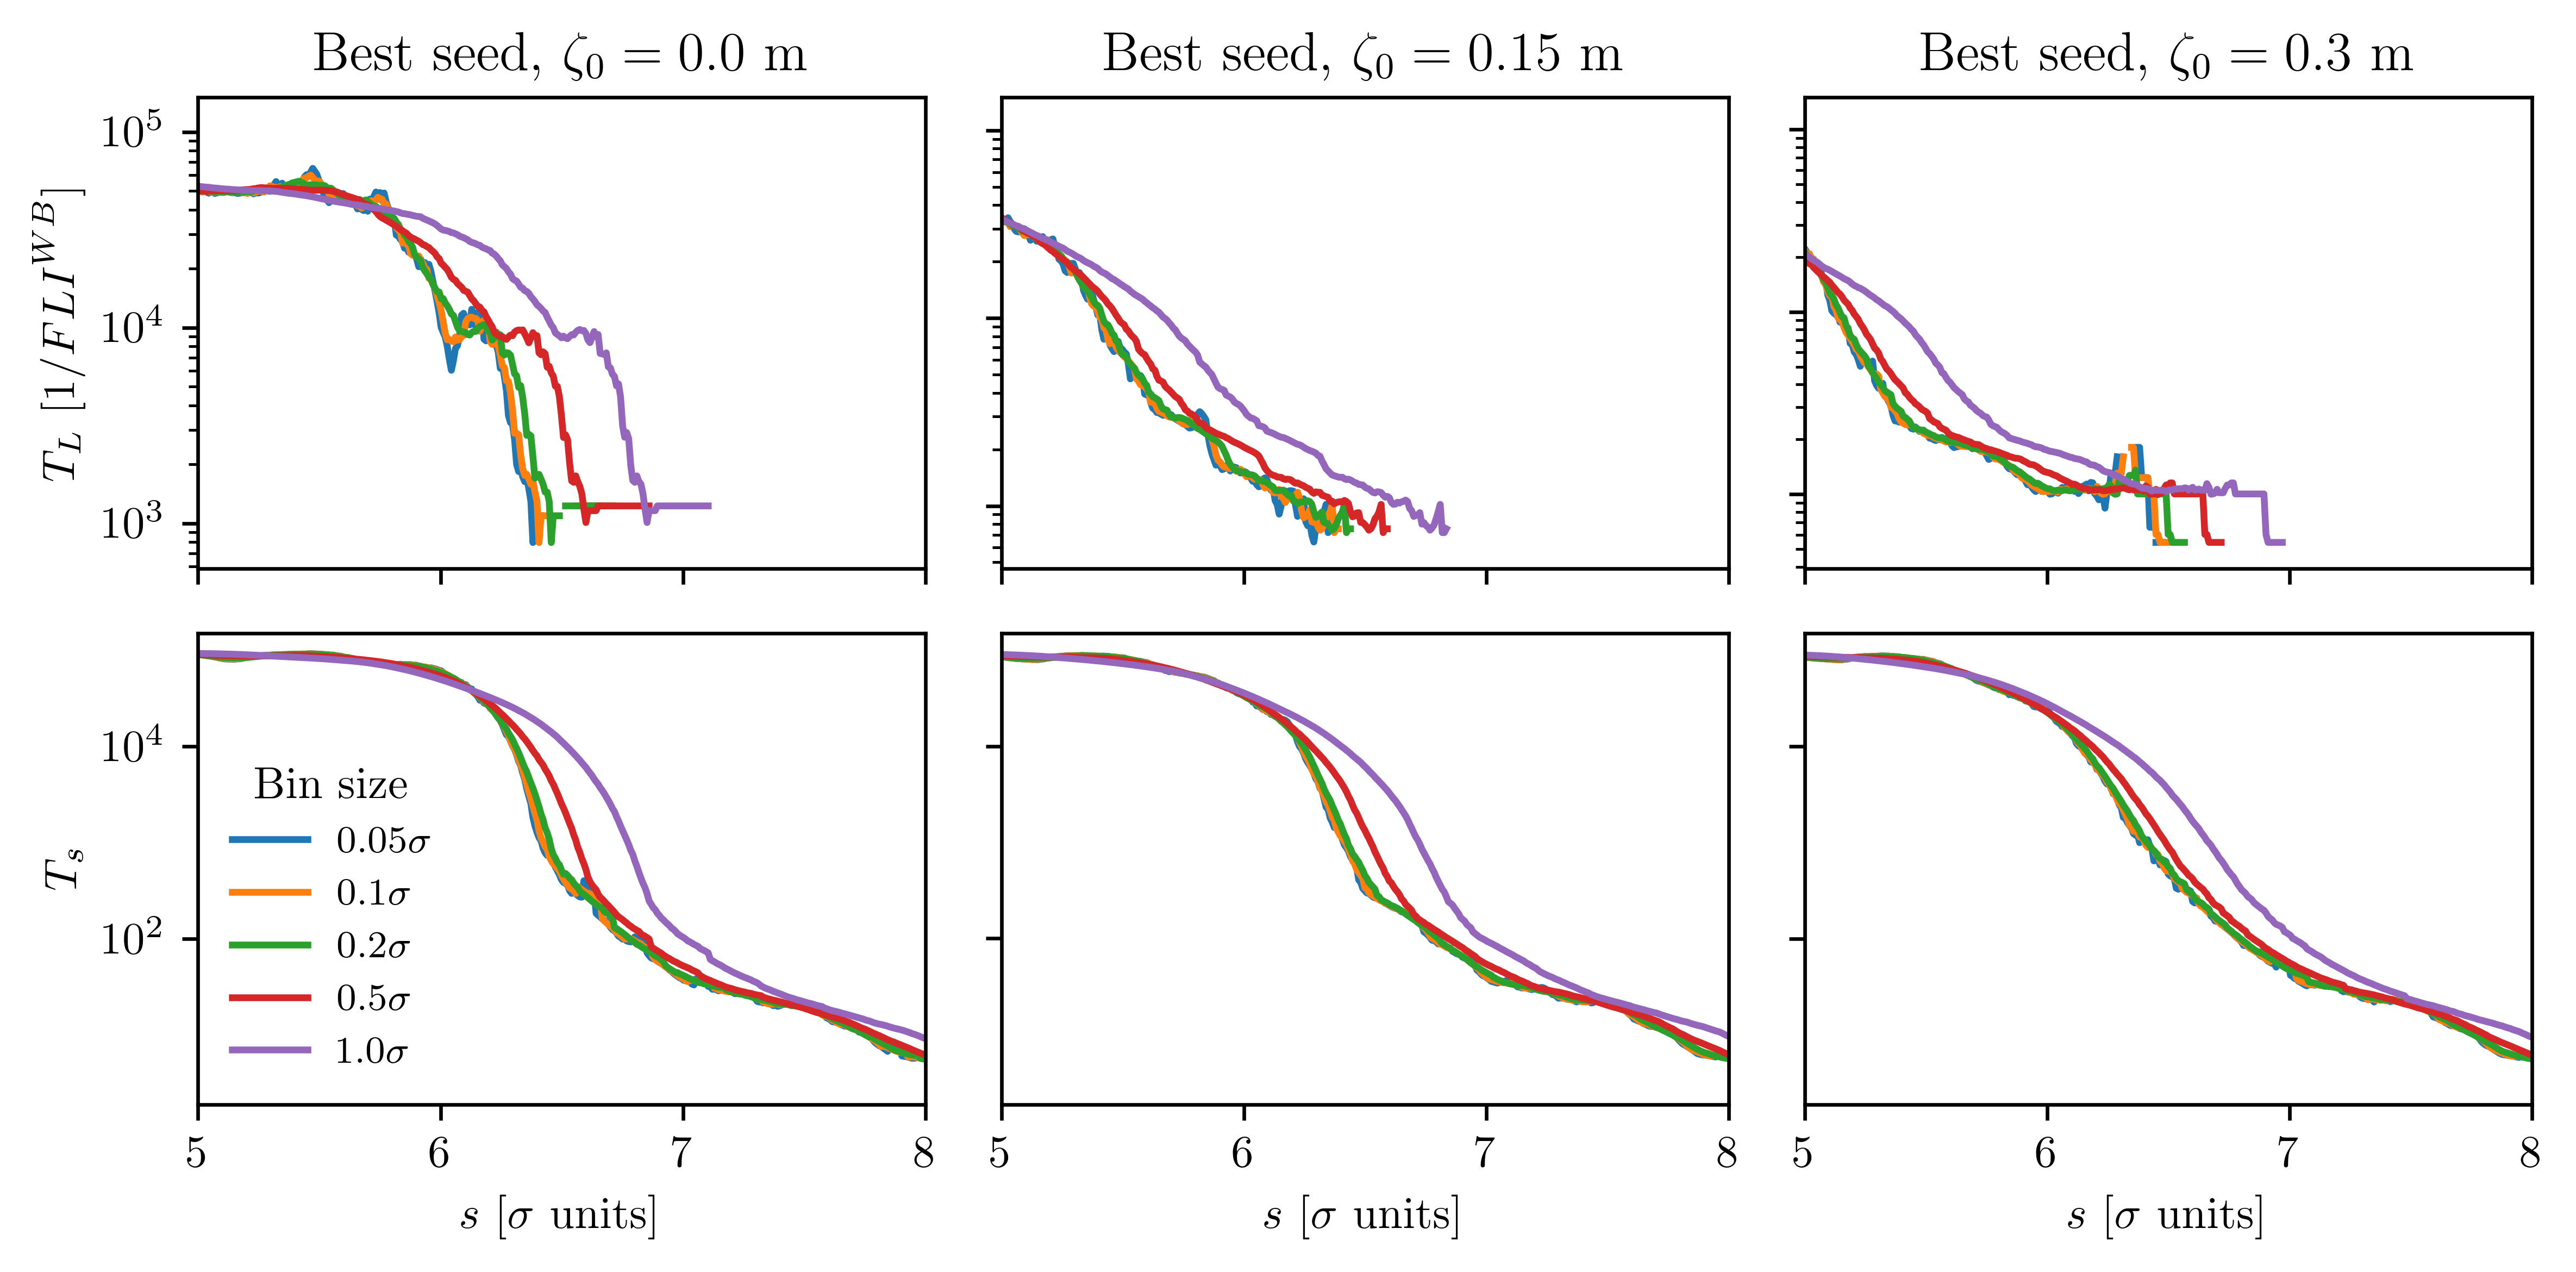
\includegraphics[width=1\textwidth]{6_lhc_dynamic_indicators/figs/lyapunov_time_vs_thickness.png}
    \caption{Mean values of $T_s$ and $T_L$ as a function of $r_0$ for a moving window of initial conditions with different values of $\Delta r$. The best compromise between statistical fluctuations and loss of information is achieved for $\Delta r = 0.2\sigma$.}
    \label{fig:ts_vs_r0}
\end{figure}

To estimate the Lyapunov time $T_L$, we can make use of both $FLI/n$ and $FLI^{{WB}}$, as they provide an estimate of the maximal Lyapunov exponent. In Fig.~\ref{fig:lyapunov_time_fli_vs_wb}, we present the results of this analysis for both $FLI/n$ and $FLI^{{WB}}$ for the same seed of the HL-LHC lattice, both evaluated at $n=10^5$. For regular orbits, the maximal Lyapunov exponent is zero, and therefore $T_L$ is infinite. For chaotic orbits, the maximal Lyapunov exponent is finite, and therefore $T_L$ is finite. However, as the $FLI/n$ and $FLI^{WB}$ dynamic indicators are evaluated at a finite time $n$, it is inevitable to observe a finite value of $T_L$ also for regular orbits. This can be observed in Fig.~\ref{fig:lyapunov_time_fli_vs_wb}, as the radiuses corresponding to regular regions of the phase space have a value plateau at an order of magnitude close to $n$. The value of $FLI^{{WB}}$, thanks to its superconvergence properties, both manages to achieve the same mean $T_L$ evaluation of $FLI/n$ for the $r_0$ corresponding to chaotic-dominant regions, and to achieve a higher value of $T_L$ for the $r_0$ corresponding to regular-dominant regions, suggesting a faster convergence to the true value of $T_L$. For this reason, we will use $FLI^{{WB}}$ in the following.

\begin{figure}
    \centering
    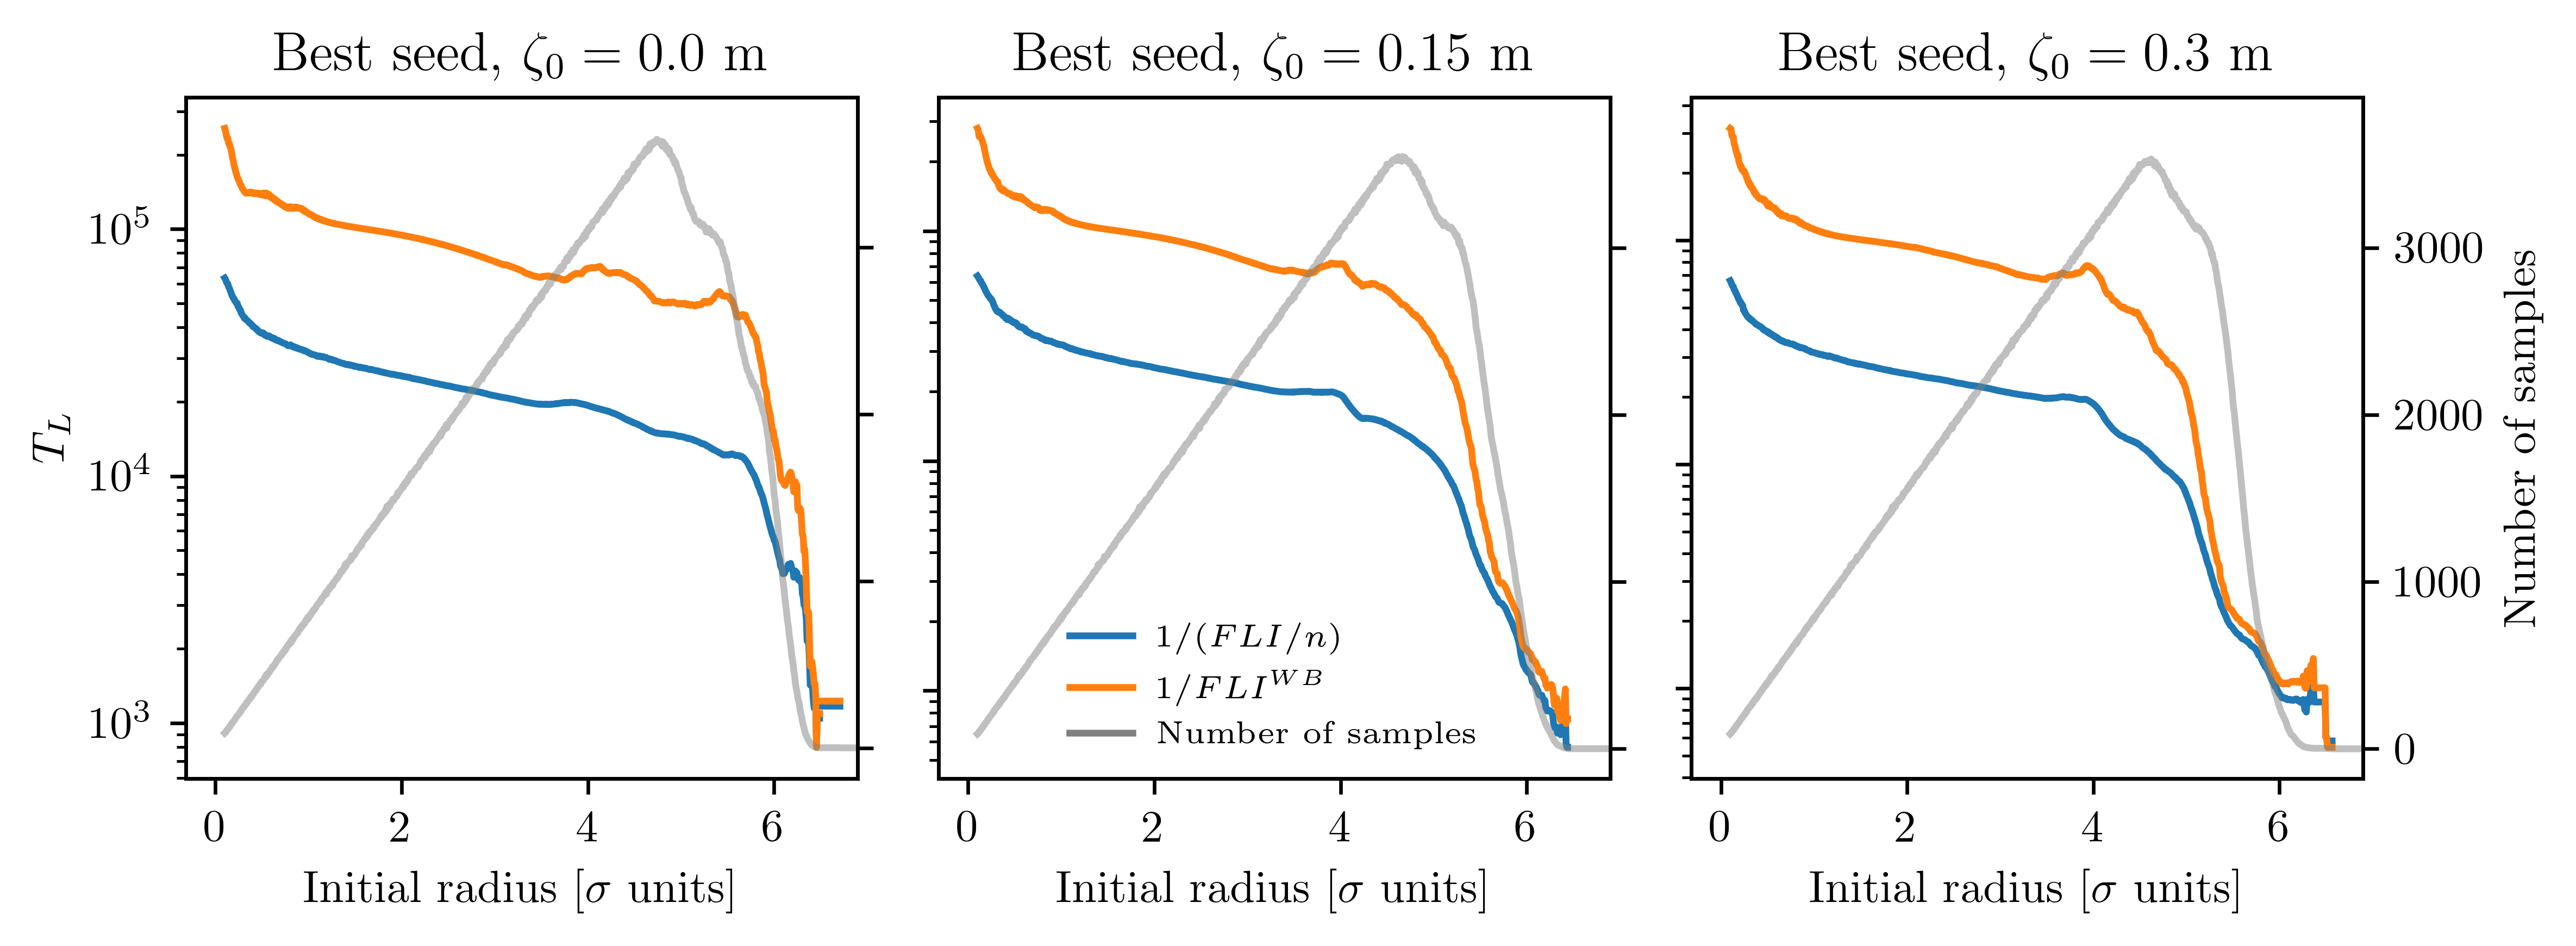
\includegraphics[width=1\textwidth]{6_lhc_dynamic_indicators/figs/lyapunov_time_vs_lyapunov_wb_time.png}
    \caption{Mean values of $T_L$ as a function of $r_0$ for a moving window of initial conditions with $\Delta r = 0.2\sigma$. The results are presented for $FLI/n$ and $FLI^{{WB}}$ evaluated at $n=10^5$. For high values of $r_0$, the two indicators provide similar results, while for low values of $r_0$, $FLI^{{WB}}$ provides a higher value of $T_L$, suggesting a faster convergence to the true value of $T_L$.}
    \label{fig:lyapunov_time_fli_vs_wb}
\end{figure}

When comparing directly $T_L$ and $T_s$, as shown in Fig.~\ref{fig:ts_vs_tl}, we can observe that the two times exhibit a similar structure with respect to $r_0$: they both exhibit a saturated plateau for low $r_0$, corresponding to the regular-dominated region, and an exponential decay over a certain radius, which varies in sharpness and position depending on the value of $\zeta_0$. In the same Figure, we also show different evaluations of $T_L$ based on $FLI^{WB}$, evaluated at different values of $n$, which explicitly show how the evaluation of $T_L$ for regular orbits increases over time, while the evaluation of $T_L$ for chaotic orbits eventually converges to its true value.

To better appreciate the value distribution observed for $T_L$ and $T_s$ at different values of $r_0$, in Fig.~\ref{fig:extra_distribution} we show as a colormap the evolution of the distribution of values from which we then evaluate the mean value. We can observe how the value distribution evolves towards a spreader distribution as $r_0$ increases. $T_s$ for low values of $r_0$ is all concentrated in a single value, which is the maximum value of tracking time.   

\begin{figure}
    \centering
    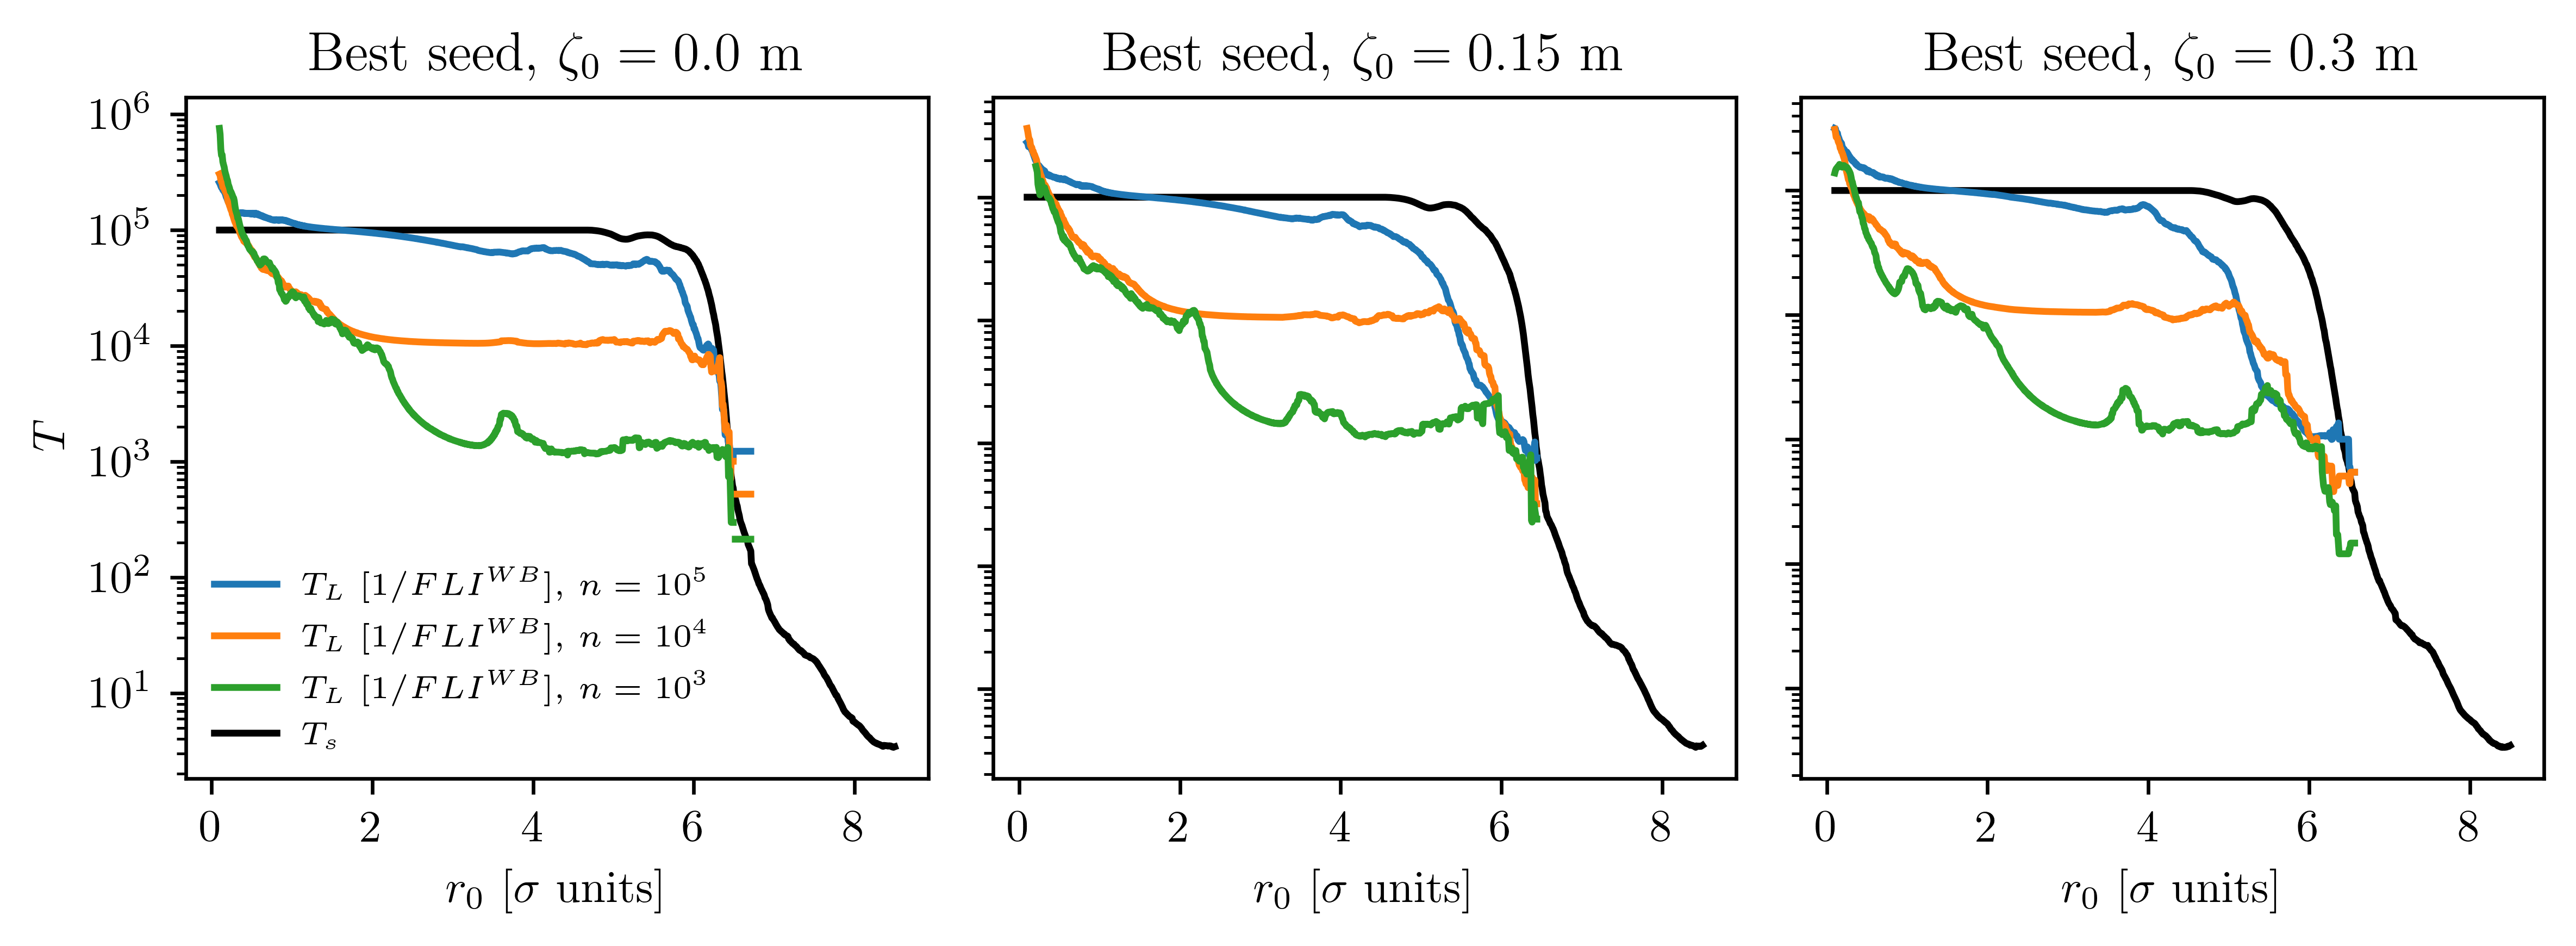
\includegraphics[width=1\textwidth]{6_lhc_dynamic_indicators/figs/lyapunov_time_vs_radius.png}
    \caption{Mean values of $T_L$ and $T_s$ as a function of $r_0$ for a moving window of initial conditions with $\Delta r = 0.2\sigma$. The values of $T_L$ are evaluated for $FLI^{{WB}}$ evaluated at three different values of $n$.}
    \label{fig:ts_vs_tl}
\end{figure}

\begin{figure}
    \centering
    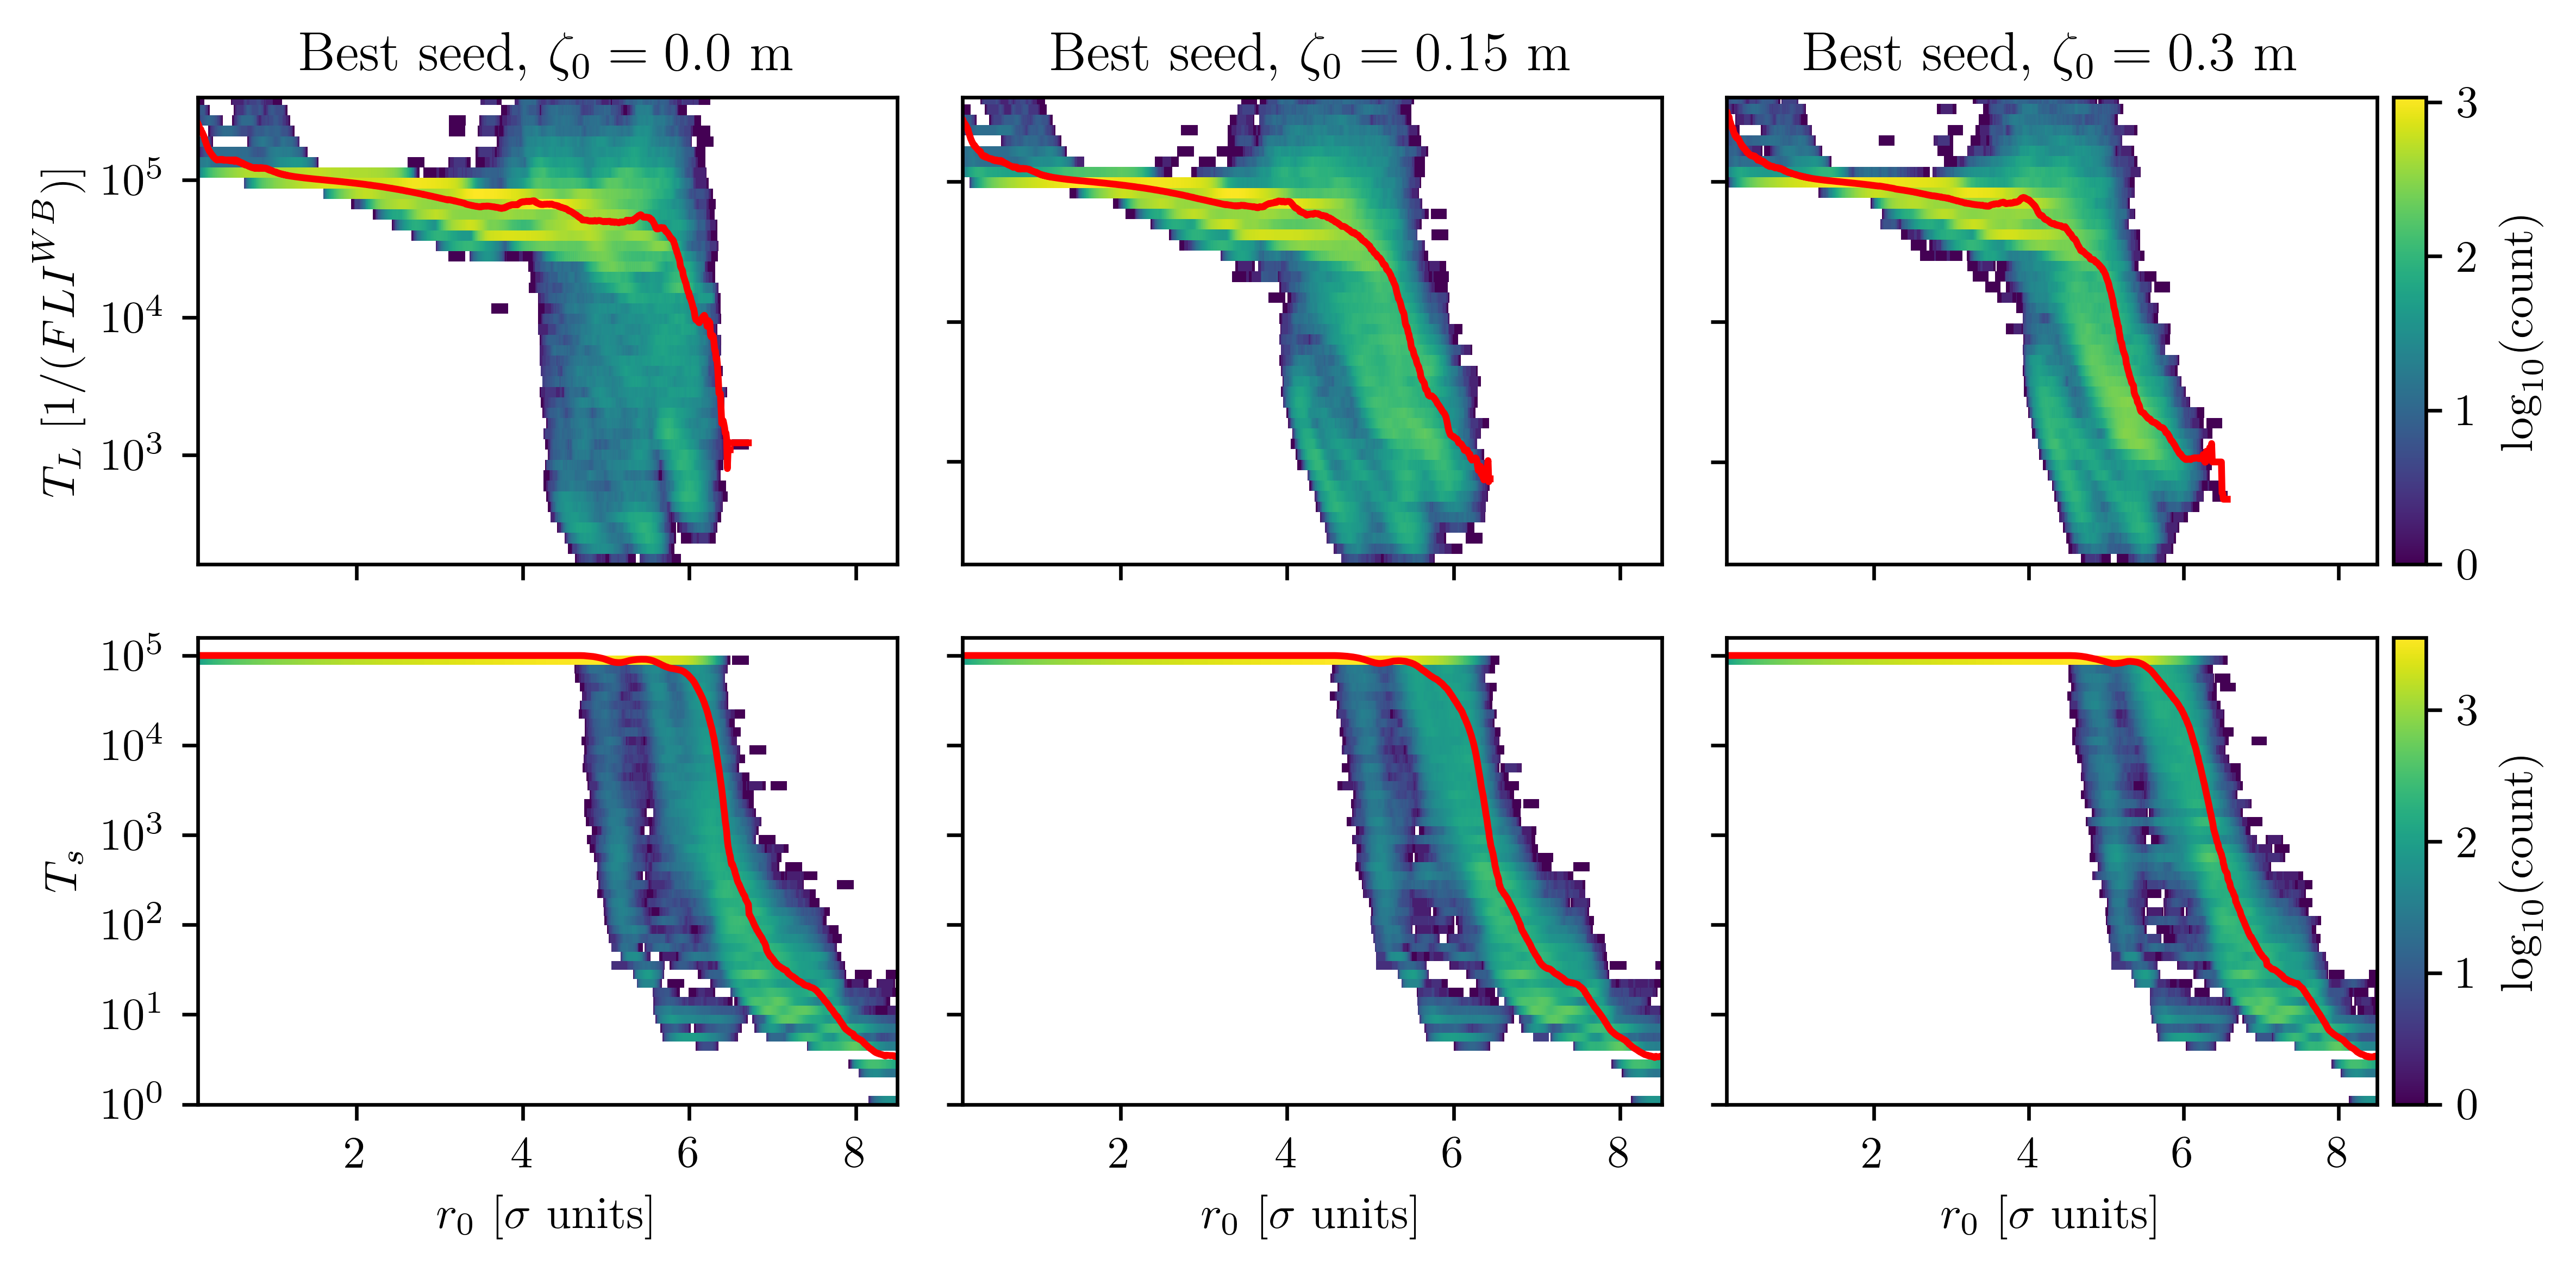
\includegraphics[width=1\textwidth]{6_lhc_dynamic_indicators/figs/dist_and_mean.png}
    \caption{Distribution of values of $T_L$ and $T_s$ as a function of $r_0$ for a moving window of initial conditions with $\Delta r = 0.2\sigma$. The red line represents the mean value of the distribution.}
    \label{fig:extra_distribution}
\end{figure}

We now want to fit a Nekhoroshev-like function
\begin{equation}
    T = T_0 \exp\left[-\left(\frac{I_0}{I_0^*}\right)^A\right]
\end{equation} 
to both $T_L$ and $T_s$, and inspect both the goodness of the fit and the evolution of the values of $T_0$, $I_\ast$, and $\kappa$ for the different combinations of seeds and values of $\zeta_0$. As this scale law ranges over multiple orders of magnitude, we consider the logarithm of $T$, and fit the following function:
\begin{equation}
    \log(T) = \log(T_0) - \left(\frac{I_0}{I_0^*}\right)^A \,.
\end{equation}
To fit the function, we first perform an initial brute force search over a grid of values of $T_0$, $I_0^*$, and $A$, and then we perform a more refined search around the best values found in the first step using the least squares method. This initial search is motivated by the non-linear nature of the fit, which makes it difficult to find the best values of the parameters with a simple gradient descent method.

As we have seen in Fig.~\ref{} and discussed previously, both evaluations of $T_L$ and $T_s$ are inevitably affected by the fact that they are evaluated on a finite number of turns $n=10^5$. Because of this, when performing the fit, we have to consider the part of the data that does not show saturation, which is the part of the data 

\subsection{Dependence of FMA from the longitudinal dynamics}

As it was pointed out in subsection~\ref{}, the chaotic structures highlighted by FMA are very different from the ones highlighted by the other dynamic indicators. This is due to the fact that the FMA indicator is sensitive in general to tune changes, which are not necessarily related to a chaotic dynamics, but might be related, for example, to the presence of tune resonances.

To further highlight this characteristic of FMA, we can observe how the indicator is particularly sensitive to the presence of longitudinal dynamics. In Fig.~\ref{fig:fma_vs_fli}, we present FMA evaluated on the same seed at the three different values of $\zeta_0$, and we compare the resulting structures and value evolution of $FLI^{WB}$. We can observe how higher values of $\zeta_0$, which lead to stronger longitudinal dynamics and modulation, cause larger differences in the structures highlighted by FMA and $FLI^{WB}$. This is due to the fact that stronger longitudinal dynamics leads to stronger modulation effects in the transverse tunes, which ultimately may lead to cases of regular orbits with varying fundamental frequencies.   

Moreover, if we compare the evolution of the value distribution of FMA, we can observe how FMA evolves into a tri-modal distribution. Differently from the other dynamic indicators, which show a tendency to create a bimodal distribution.

\begin{figure}[ht]
    \centering
    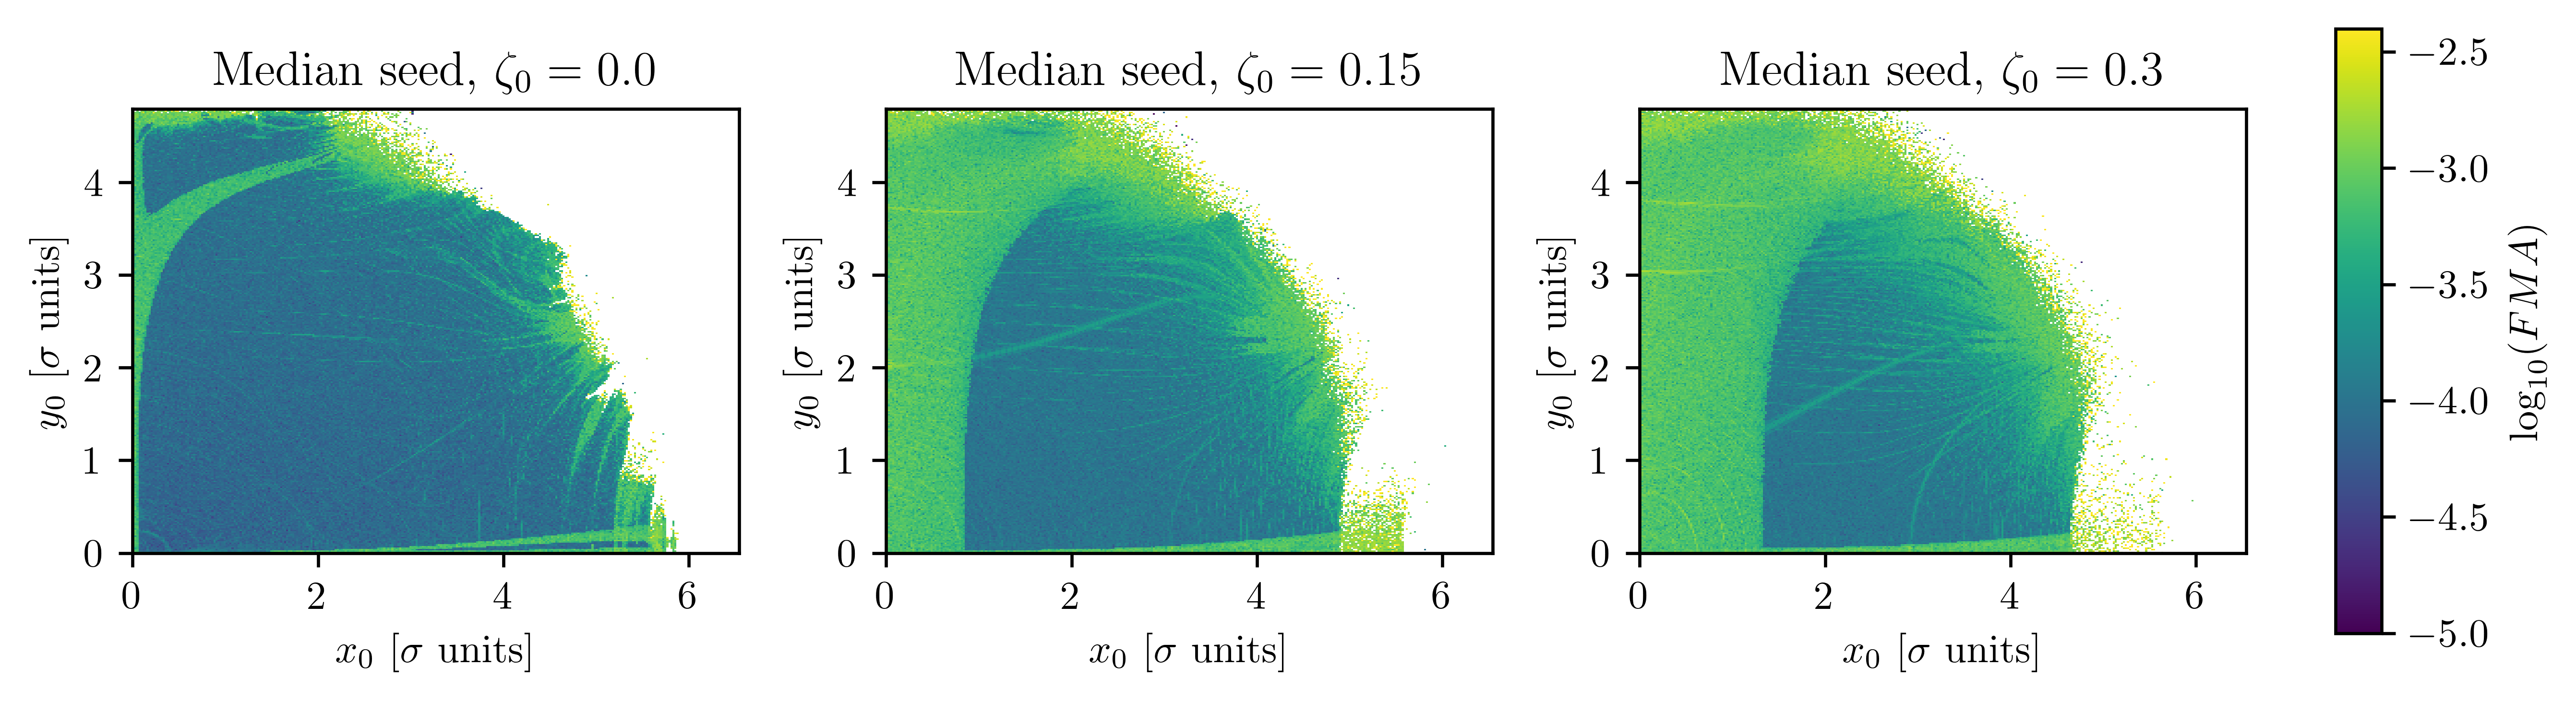
\includegraphics[width=1.0\textwidth]{6_lhc_dynamic_indicators/figs/FMA.png}
    \caption{(Top) $\log_{10}(\mathrm{FMA})$ and $\log_{10}(\mathrm{FLI}^{WB})$ evaluated on the same seed at three different values of $\zeta_0$. Higher values of $\zeta_0$ yields larger differences between the regions highlighted by the two indicators. (Bottom) Evolution of the value distribution over time of $\log_{10}(\mathrm{FMA})$ and $\log_{10}(\mathrm{FLI}^{WB})$. While $\mathrm{FLI}^{WB}$ shows a clear tendency to create a bimodal distribution, $\mathrm{FMA}$ instead evolves into a tri-modal distribution.}
    \label{fig:fma_vs_fli}
\end{figure}

\subsection{General performances of REM}


\subsection{Different subspace choices for GALI$^{(k)}$}